\chapter{Resultados}\label{cap:resultados}
\graphicspath{{chapter-07/img-cap07/}}

\section{Projetil inerte (sem \textit{Base Bleed})}\label{sec:resultados-sem-basebleed}

Os valores encontrados para o coeficiente de arrasto aerodinâmico em um projetil de artilharia sem uso de \textit{Base Bleed} foram desenvolvidos a partir do modelo SST \(\kappa-\omega\), como visto na \autoref{fig:cd-sembasebleed-comparacao}. As curvas de arrasto foram desenvolvidas com base nas malhas citadas na \autoref{tab:tabela-malhas-inicial} e foram comparadas com os resultados obtidos em simulação computacional desenvolvida por \citeauthor{Mahmoud2009}. 

\begin{figure}[!ht]
	\centering
	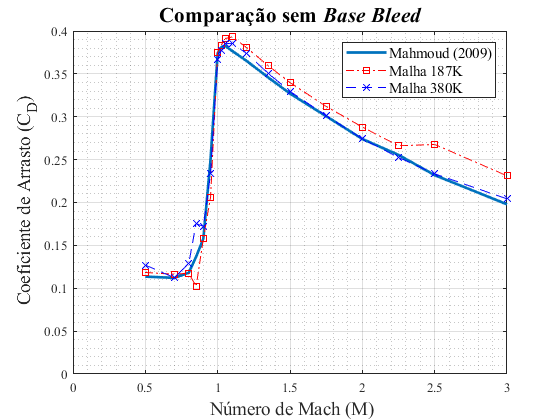
\includegraphics[width=0.75\textwidth]{cd-sembasebleed-comparacao.png}
	\caption{Coeficiente de Arrasto \(C_{D}\) em função do número de Mach (sem BB)}
	\label{fig:cd-sembasebleed-comparacao}
\end{figure}

Através do que é demonstrado na Figura \autoref{fig:cd-sembasebleed-comparacao}, percebe-se que a curva referente a malha com \num{380000} elementos (380K) se aproximou consideravelmente da referência. Por esta razão, a implementação do domínio computacional foi considerada válida para as próximas análises com a tecnologia \textit{Base Bleed} como condição de contorno.

\begin{figure}[!ht]
	\centering
	\begin{subfigure}[b]{0.47\textwidth}
        \centering
        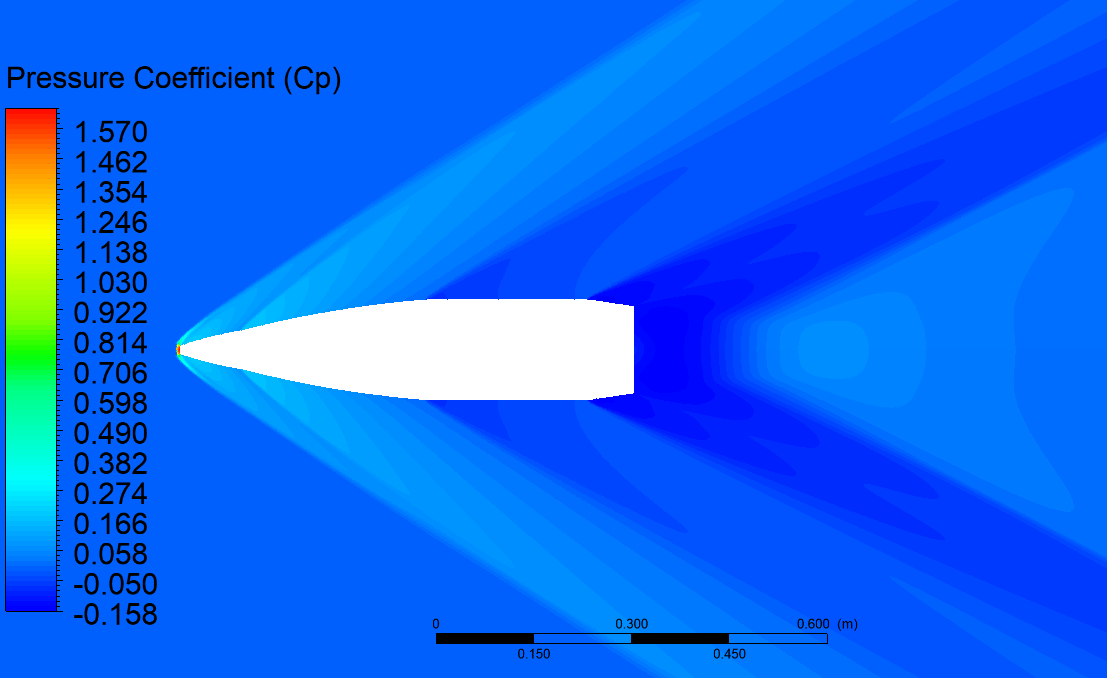
\includegraphics[height=5cm,width=\textwidth]{contorno-pressao.png}
        \caption{Contornos de Pressão}
        \label{fig:contorno-pressao-sembasebleed}
    \end{subfigure}
    \hfill
	\begin{subfigure}[b]{0.47\textwidth}
        \centering
        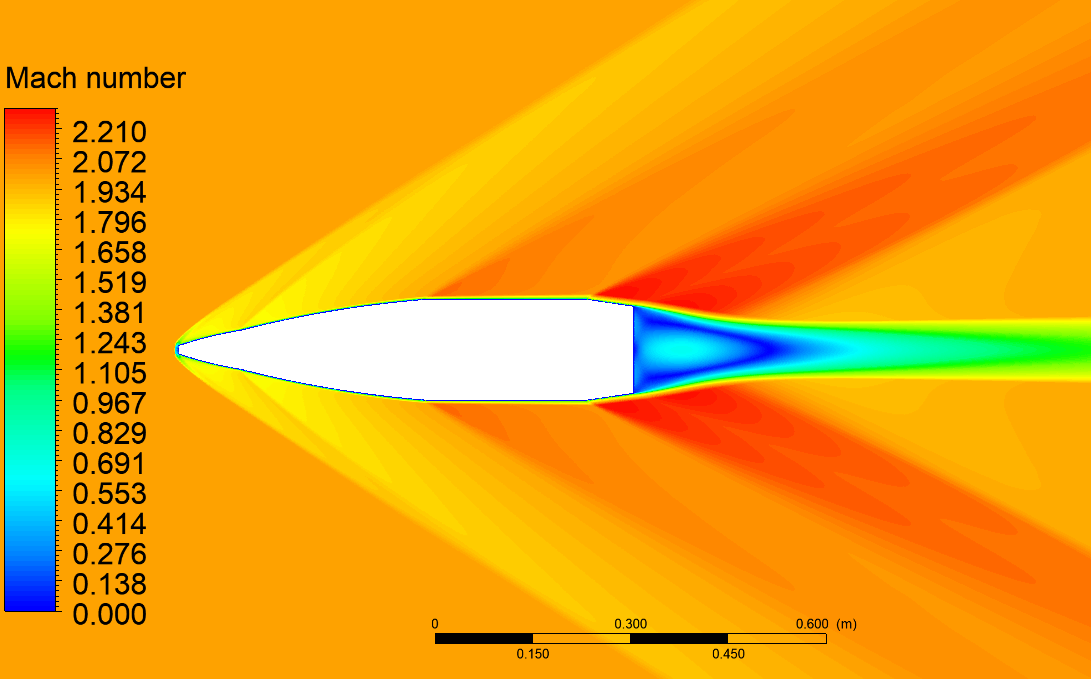
\includegraphics[height=5cm,width=\textwidth]{contorno-velocidade.png}
        \caption{Contornos de Velocidade}
        \label{fig:contorno-velocidade-sembasebleed}
    \end{subfigure}
	\caption{Projetil sob regime de velocidade igual a Mach \num{2}}
	\label{fig:contornos-pressao-velocidade-sembasebleed}
\end{figure}

Antes de iniciar as validações das simulações que incluem o efeito \textit{Base Bleed}, é necessário observar a \autoref{fig:contornos-pressao-velocidade-sembasebleed}, pois os contornos de pressão (\autoref{fig:contorno-pressao-sembasebleed}) e de velocidade (\autoref{fig:contorno-velocidade-sembasebleed}) demonstram o escoamento do ar em torno do projetil. Além da onda de choque causada pela velocidade supersônica (M = \num{2,0}), existe uma região de baixa pressão na base da munição cuja consequência é criar uma região de recirculação com baixas velocidades. Contudo, é a partir da \autoref{fig:corrente-velocidade-sembasebleed} que se examina com maiores detalhes o comportamento desta recirculação outrora citada.

\begin{figure}[!ht]
    \centering
    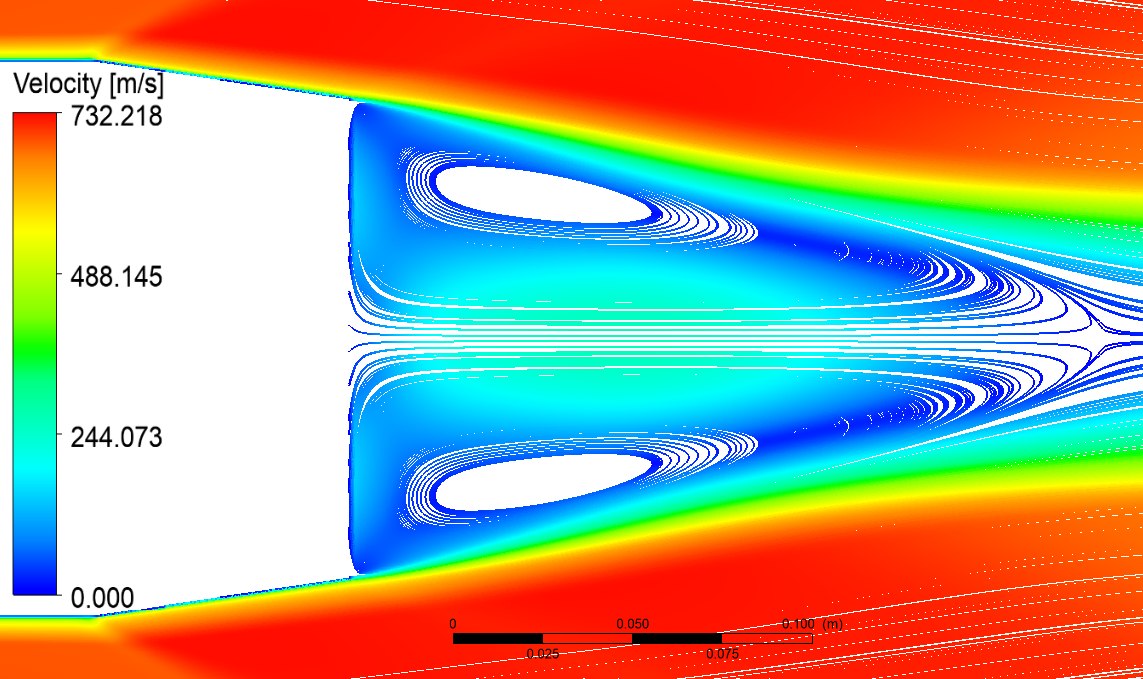
\includegraphics[height=5cm,width=0.5\textwidth]{corrente-velocidade-off.png}
    \caption{Linhas de corrente para a velocidade sob regime M = \num{2,0}}
    \label{fig:corrente-velocidade-sembasebleed}
\end{figure}

\section{Projetil ativo (com \textit{Base Bleed})}\label{sec:resultados-com-basebleed}

A Tabela \ref{tab:tabela-malhas-secundaria}, presente na Seção \ref{sec:geracao-malha}, demonstra as malhas testadas para o projetil ativo. A malha com \num{380000} elementos foi utilizada como referência, tendo em vista a convergência dos resultados com valores de trabalhos anteriores \cite{Mahmoud2009}. Com estas malhas foram feitos testes de convergência, em dois regimes de velocidade (Mach igual a \numlist{1,0;2,0}), cujos resultados são apresentados na \autoref{tab:tabela-malhas-convergencia}. Em ambos os casos o modelo SST \(\kappa-\omega\) foi usado para descrever a turbulência. A condição de contorno "Entrada do \textit{Base Bleed}"{} considerou a saída dos gases com a seguinte configuração: \(\phi_{BB} = \qty{50,8}{\milli\metre}; \Dot{m}_{BB} = \qty{0,030}{\kilogram\per\second}; T_{BB} = \qty{2306,15}{\kelvin}\).

\begin{table}[ht]
\centering
\caption[Teste de convergência (com \textit{Base Bleed})]{Teste de convergência (com \textit{Base Bleed})}
\vspace{0.5cm}
\begin{tabular}{c|c|c|c|c}
\multicolumn{5}{c}{Segundo Teste de Convergência} \\
\hline 
Número de elementos & \(C_{D}\) (M = \num{1}) & Diferença & \(C_{D}\) (M = \num{2}) & Diferença\\ 
\hline
\num{380000} & 0,32784 & -- & 0,26330 & --\\
\num{453600} & 0,33064 & \qty{0,854}{\percent} & 0,26364 & \qty{0,129}{\percent}\\
\num{514800} & 0,32912 & \qty{0,390}{\percent} & 0,26185 & \qty{0,551}{\percent}\\
\num{566550} & 0,32656 & \qty{0,394}{\percent} & 0,26143 & \qty{0,710}{\percent}\\
\end{tabular}
\label{tab:tabela-malhas-convergencia}
\fonte{Autor.}
\end{table}

Para o projetil em velocidade sônica (M = \num{1,0}), a maior diferença percentual ficou na ordem de \qty{0,85}{\percent}, enquanto que para M = \num{2,0} o maior desvio foi de aproximadamente \qty{0,7}{\percent}, o que denota quase nenhuma diferença nos resultados mesmo aumentando significativamente o número de elementos. Desta forma, o custo computacional para resolver a malha com \num{380000} elementos é suficiente para predizer o coeficiente de arrasto.

\subsection{Influência no diâmetro de saída do \textit{Base Bleed}} \label{subsec:resultados-com-basebleed-diametros}

Outro parâmetro considerado foi o aumento do diâmetro da saída do bocal (ver \autoref{tab:tabela-vazoes-por-diametro}), de \qtyrange{25,4}{50,8}{\millimetre} (de \qtyrange{1}{2}{\polegada}). A temperatura na condição de contorno "Entrada do \textit{Base Bleed}"{} foi fixada em \(T_{BB} = \qty{2306,15}{\kelvin}\). Desta forma, a Figura \ref{fig:comparacao-bb-diametro-2pol} demonstra uma redução do coeficiente de arrasto para um diâmetro de \qty{2}{\polegada}, enquanto que a Figura \ref{fig:comparacao-bb-diametro-1pol} mostrou que o diâmetro de \qty{1}{\polegada} aumentou o perfil de arrasto, se comparado ao sistema BB desativado.

\begin{figure}[!ht]
	\centering
	\begin{subfigure}[b]{0.47\textwidth}
    	\centering
    	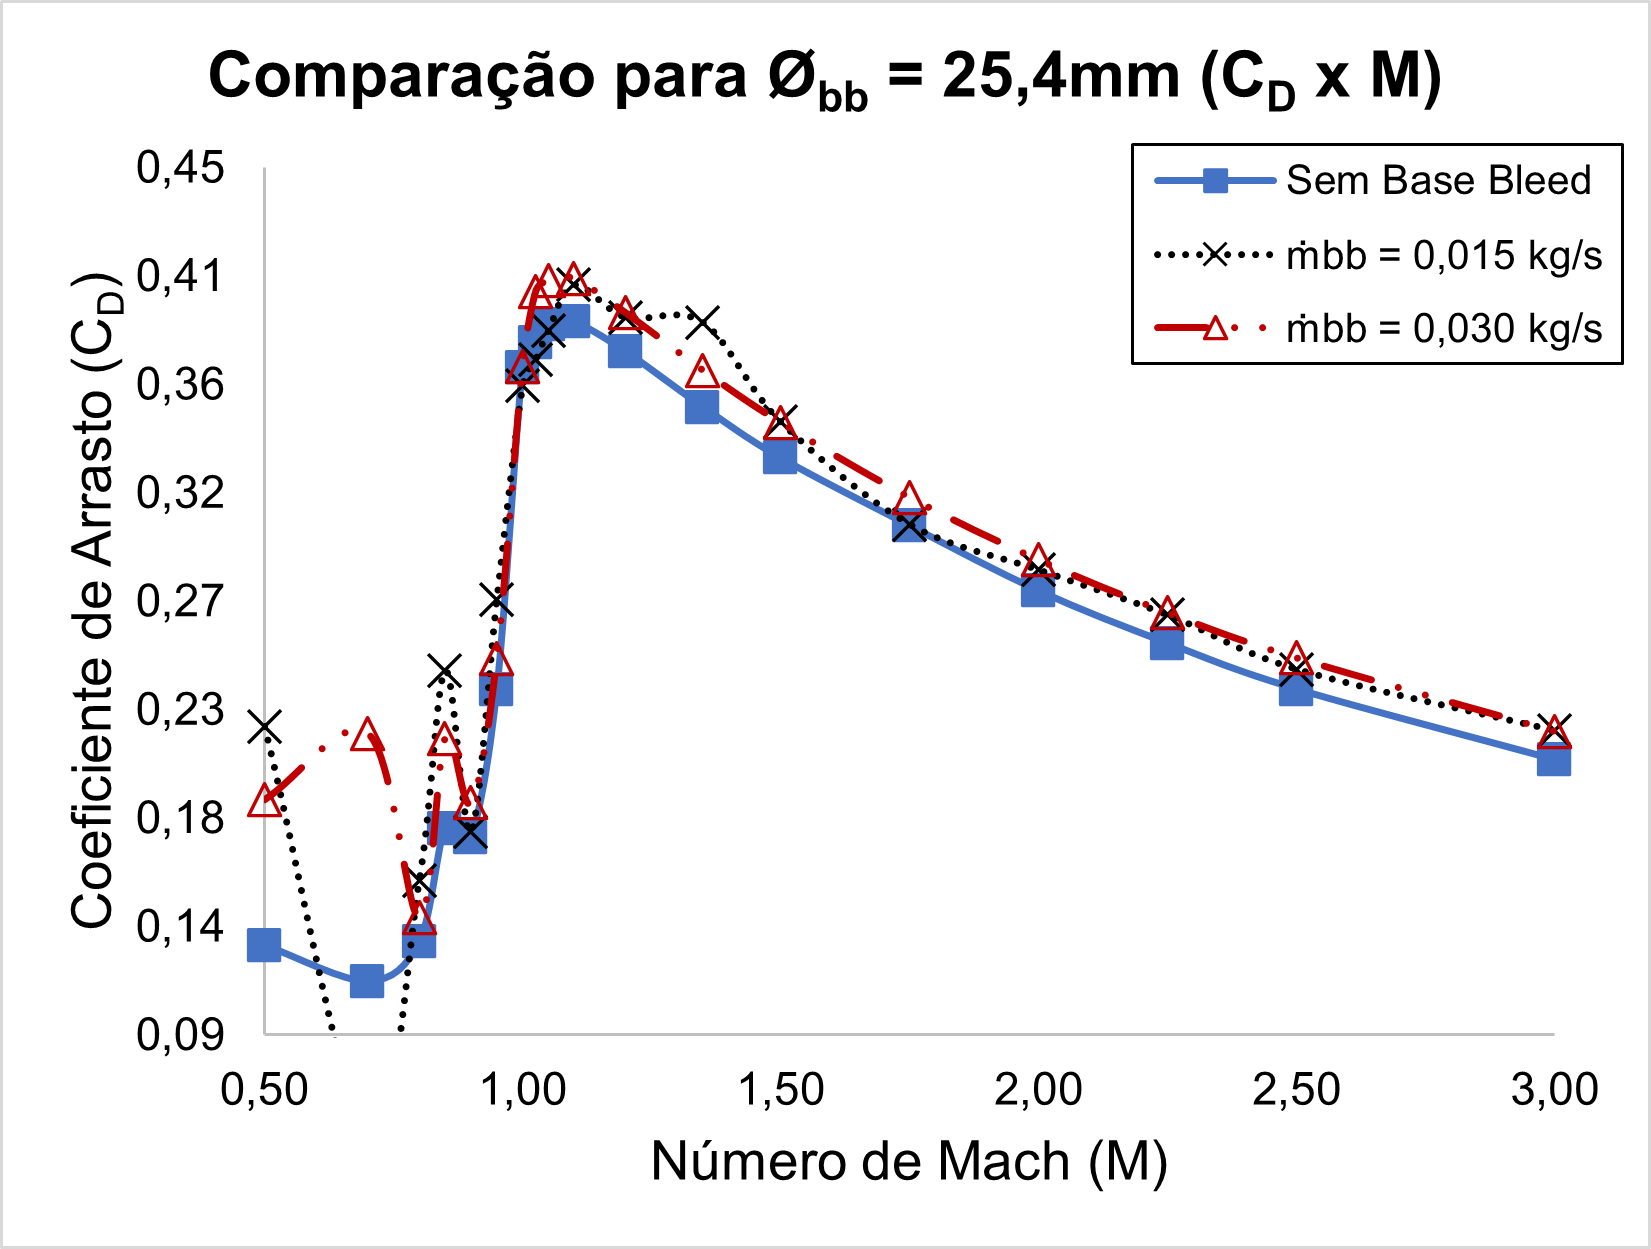
\includegraphics[width=\textwidth]{cd-combasebleed-diametro-1pol.png}
    	\caption{Saída do bocal - \(\phi_{BB}\) = \qty{25,4}{\millimetre}}
    	\label{fig:comparacao-bb-diametro-1pol}
    \end{subfigure}
    \hfill
	\begin{subfigure}[b]{0.47\textwidth}
    	\centering
    	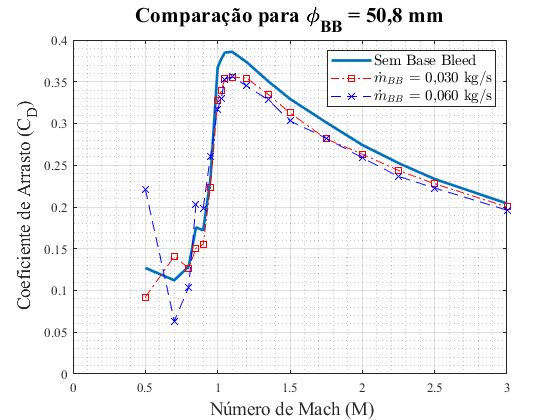
\includegraphics[width=\textwidth]{cd-combasebleed-diametro-2pol.png}
    	\caption{Saída do bocal - \(\phi_{BB}\) = \qty{50,8}{\millimetre}}
    	\label{fig:comparacao-bb-diametro-2pol}
    \end{subfigure}
	\caption{Influência do diâmetro sobre o coeficiente de arrasto.}
	\label{fig:comparacao-bb-diametro-vazoes}
\end{figure}

Há de se notar uma oscilação presente nas curvas de arrasto no regime subsônico com o \textit{base bleed} funcionando, especialmente na faixa M < \num{0,8}. A escolha das vazões de \qty{0,015}{\kilogram\per\second} e \qty{0,060}{\kilogram\per\second} foi para garantir a conservação da velocidade ao aumentar em 4 vezes a área de saída dos gases do \textit{Base Bleed}. Ainda analisando os resultados pelas vazões mássicas, atesta-se da \autoref{fig:comparacao-bb-diametro-vazoes} que os coeficientes de arrasto sofreram redução em ambos os casos, embora pouco relevantes.

Para entender o que ocorreu para acrescentar o arrasto nos projetis com diâmetro de saída do \textit{Base Bleed} iguais a \qty{1}{"} \(\left(\phi_{BB} = \qty{25,4}{\millimetre}\right)\), a \autoref{fig:influencia-diametro-vazao-1pol} apresenta os campos de pressão e velocidade sob regime M = \num{2,0}. Conforme esperado pela literatura, as Figuras \ref{fig:contorno-pressao-bb-1pol-vazao0015} e \ref{fig:contorno-pressao-bb-1pol-vazao0030} demonstram o campo de pressão à jusante da base do projetil, que está abaixo do valor prescrito da região denominada "Escoamento livre"{} do domínio computacional. Tanto na \autoref{fig:contorno-pressao-bb-1pol-vazao0015} quanto na \autoref{fig:contorno-pressao-bb-1pol-vazao0030} não há um aumento significativo da pressão atmosférica na região, apesar da diferenciação do campo de velocidades ser demonstrada pelas Figuras \ref{fig:contorno-velocidade-bb-1pol-vazao0015} e \ref{fig:contorno-velocidade-bb-1pol-vazao0030}. Contudo, a apresentação do campo de velocidades da \autoref{fig:contorno-velocidade-bb-1pol-vazao0030} reflete uma vazão mássica excedente que aumenta a força de arrasto.

As Figuras \ref{fig:corrente-velocidade-bb-1pol-vazao0015} e \ref{fig:corrente-velocidade-bb-1pol-vazao0030} mostram as linhas de corrente para a velocidade nas duas condições impostas para o sistema BB com \qty{1}{\polegada}. Da \autoref{fig:corrente-velocidade-bb-1pol-vazao0015} se conclui que a injeção de gases nessa vazão mássica produz nenhum efeito significativo no que diz respeito ao deslocamento da região primária de recirculação e da formação da recirculação anular.

\begin{figure}[!ht]
	\centering
	\begin{subfigure}[b]{0.47\textwidth}
        \centering
        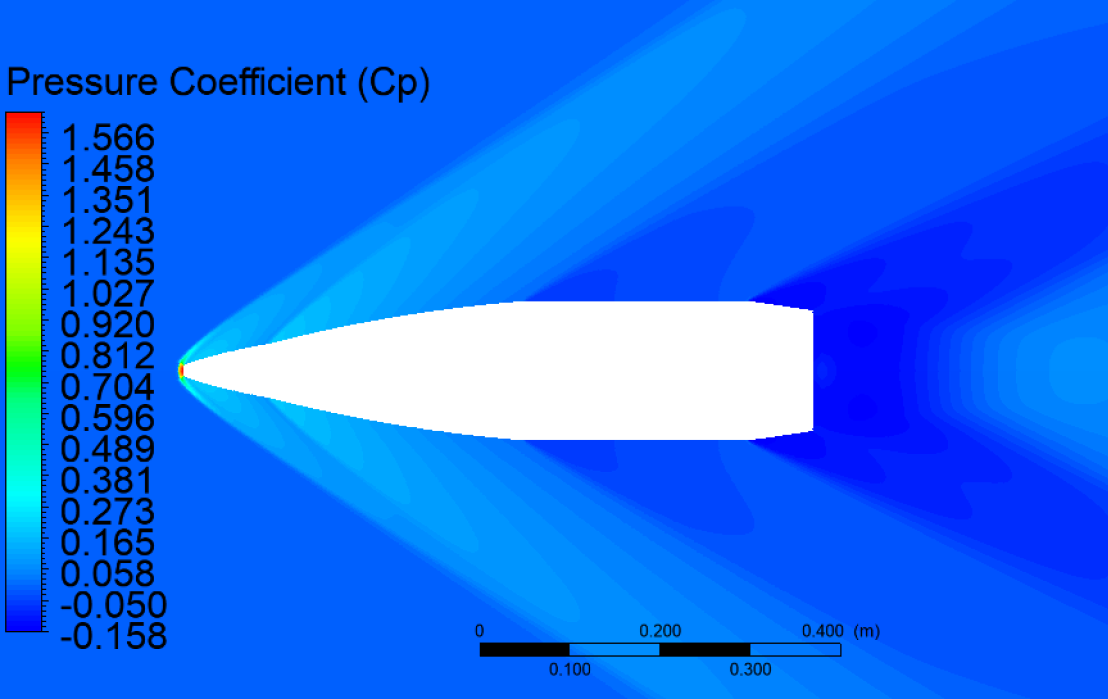
\includegraphics[height=5cm,width=\textwidth]{contorno-pressao-2306K-vazao-0015-1pol.png}
        \caption{Contornos de Pressão - \(\Dot{m}_{BB}\) = \qty{0,015}{\kilogram\per\second}}
        \label{fig:contorno-pressao-bb-1pol-vazao0015}
    \end{subfigure}
    \hfill
    \begin{subfigure}[b]{0.47\textwidth}
        \centering
        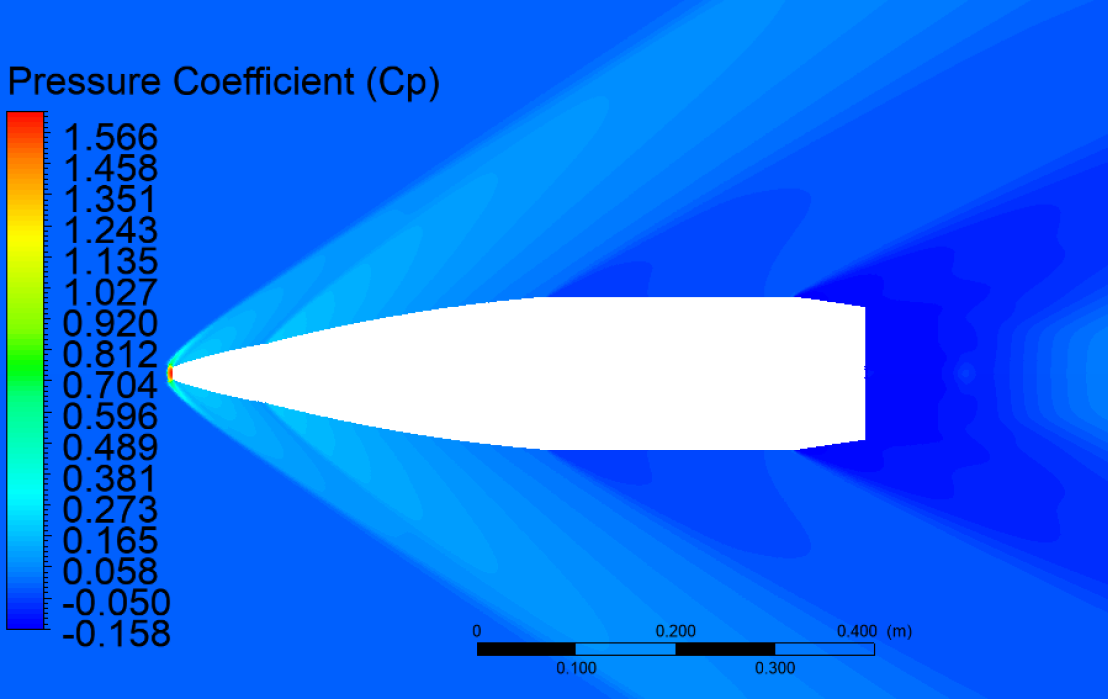
\includegraphics[height=5cm,width=\textwidth]{contorno-pressao-2306K-vazao-0030-1pol.png}
        \caption{Contornos de Pressão - \(\Dot{m}_{BB}\) = \qty{0,030}{\kilogram\per\second}}
        \label{fig:contorno-pressao-bb-1pol-vazao0030}
    \end{subfigure}
    \hfill
    \begin{subfigure}[b]{0.47\textwidth}
        \centering
        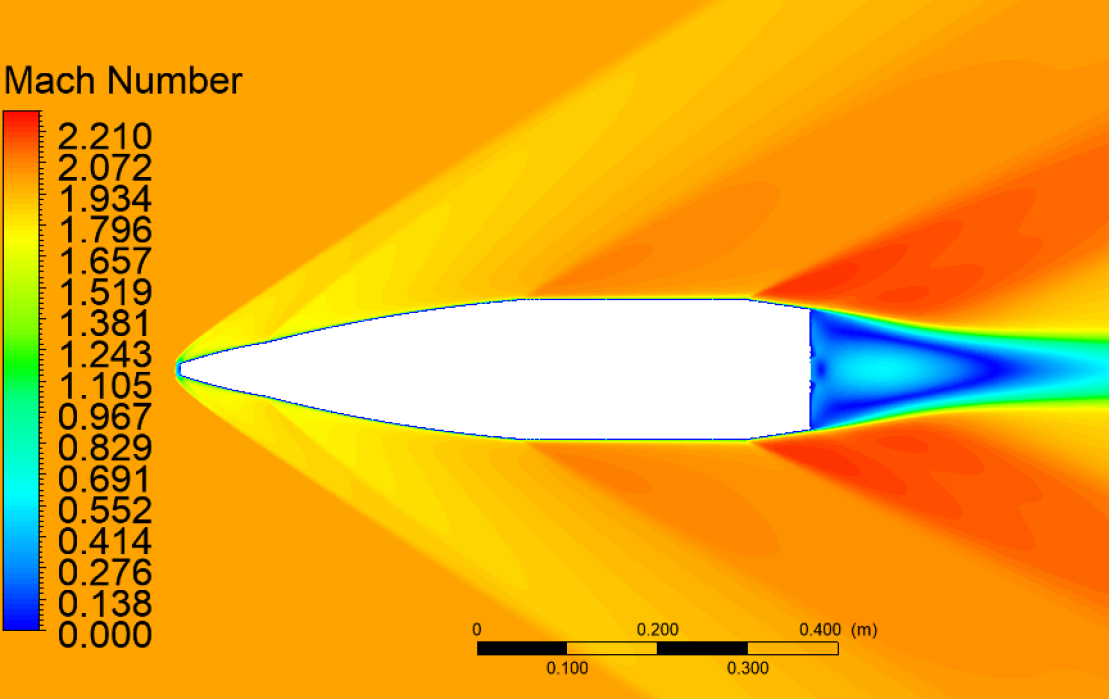
\includegraphics[height=5cm,width=\textwidth]{contorno-velocidade-2306K-vazao-0015-1pol.png}
        \caption{Cont. de Velocidade - \(\Dot{m}_{BB}\) = \qty{0,015}{\kilogram\per\second}}
        \label{fig:contorno-velocidade-bb-1pol-vazao0015}
    \end{subfigure}
    \hfill
	\begin{subfigure}[b]{0.47\textwidth}
        \centering
        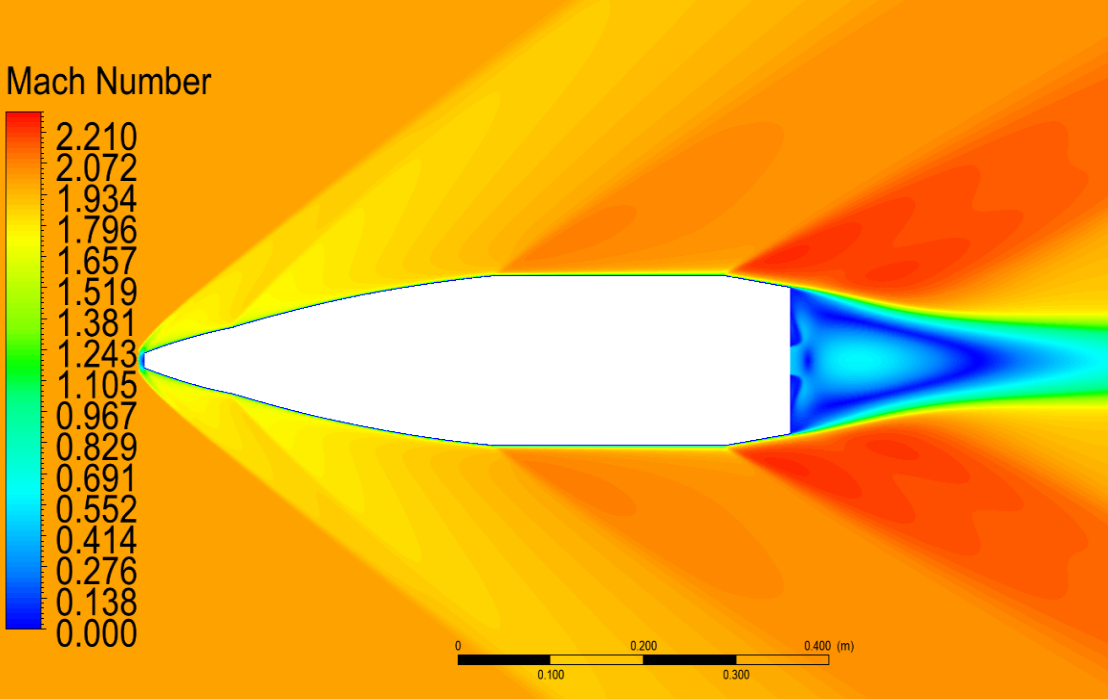
\includegraphics[height=5cm,width=\textwidth]{contorno-velocidade-2306K-vazao-0030-1pol.png}
        \caption{Cont. de Velocidade - \(\Dot{m}_{BB}\) = \qty{0,030}{\kilogram\per\second}}
        \label{fig:contorno-velocidade-bb-1pol-vazao0030}
    \end{subfigure}
    \hfill
    \begin{subfigure}[b]{0.47\textwidth}
        \centering
        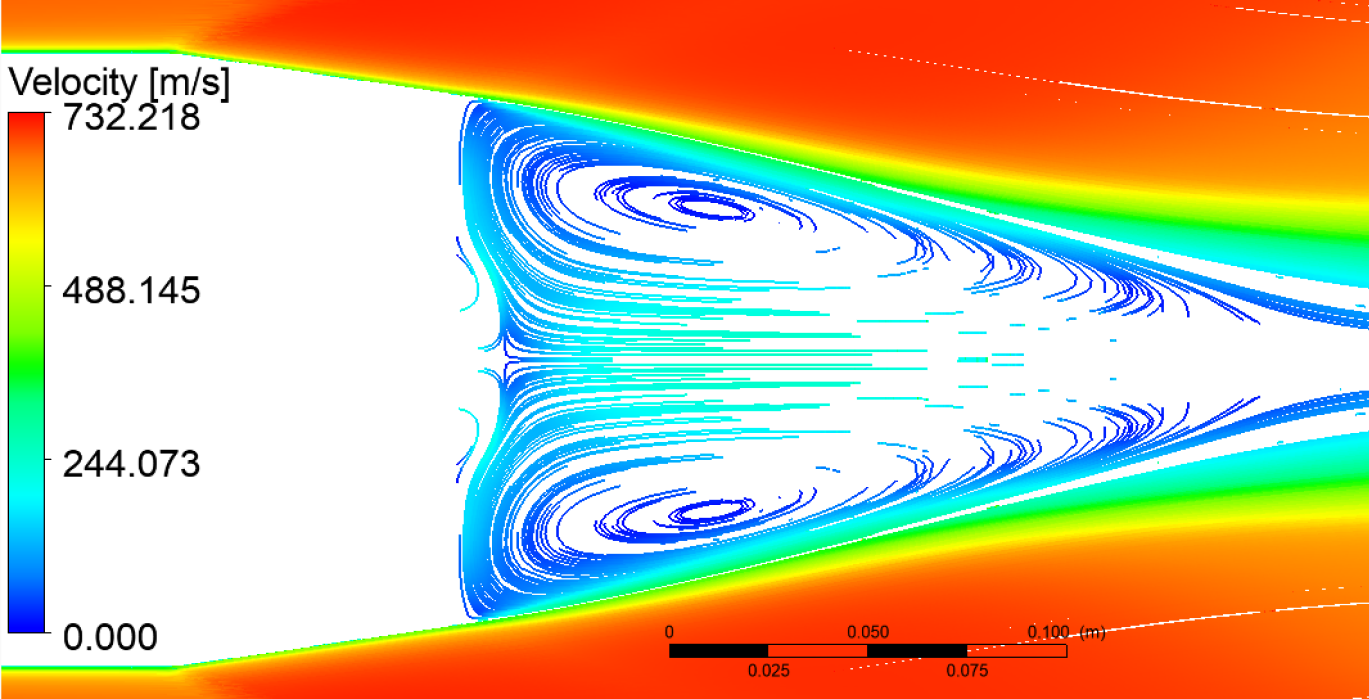
\includegraphics[height=5cm,width=\textwidth]{corrente-velocidade-2306K-vazao-0015-1pol.png}
        \caption{Linhas de corrente - \(\Dot{m}_{BB}\) = \qty{0,015}{\kilogram\per\second}}
        \label{fig:corrente-velocidade-bb-1pol-vazao0015}
    \end{subfigure}
    \hfill
    \begin{subfigure}[b]{0.47\textwidth}
        \centering
        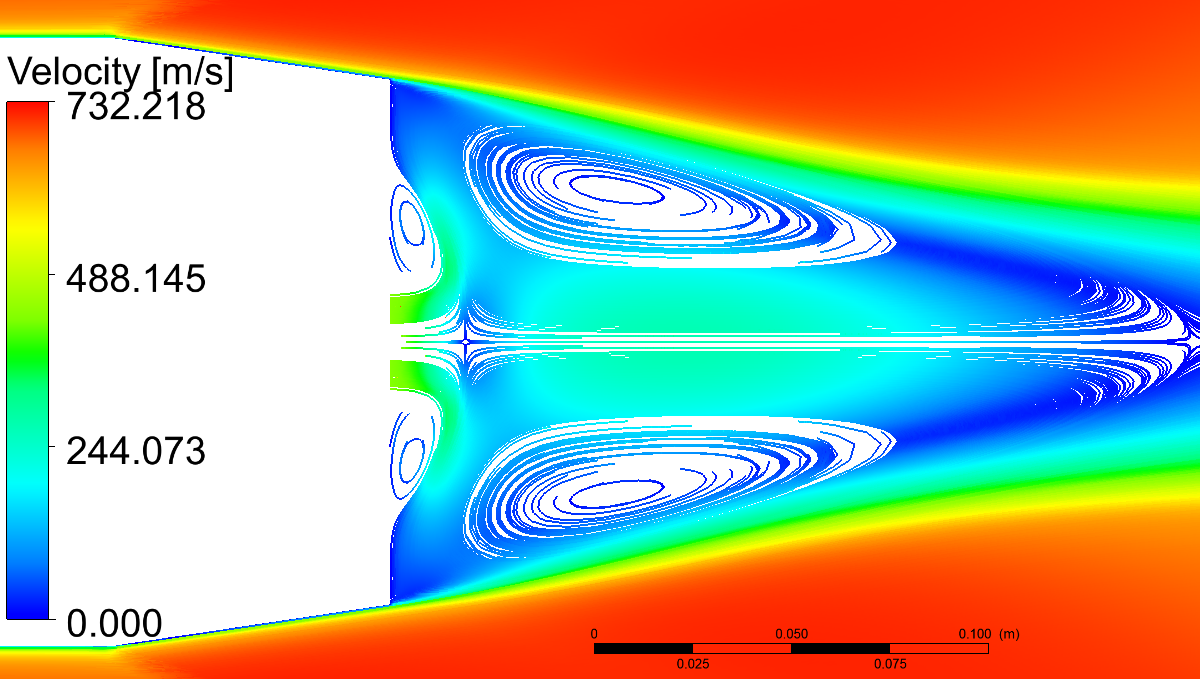
\includegraphics[height=5cm,width=\textwidth]{corrente-velocidade-2306K-vazao-0030-1pol.png}
        \caption{Linhas de corrente - \(\Dot{m}_{BB}\) = \qty{0,030}{\kilogram\per\second}}
        \label{fig:corrente-velocidade-bb-1pol-vazao0030}
    \end{subfigure}
	\caption{Projetil sob diferentes condições de vazão mássica sob regime M = \num{2,0} \(\left(\phi_{BB} = \qty{25,4}{\millimetre}; T_{BB} = \qty{2306,15}{\kelvin}\right)\)}
	\label{fig:influencia-diametro-vazao-1pol}
\end{figure}

O passo seguinte foi apresentar o escoamento no entorno do projetil assumindo que o diâmetro de saída do bocal, \(\phi_{BB}\), seja igual a 50,8 mm. Assim como na \autoref{fig:influencia-diametro-vazao-1pol}, a velocidade do meio livre foi definida como M = \num{2,0} para os contornos de pressão e de velocidade, além das linhas de corrente, sendo todos esses perfis vistos na \autoref{fig:influencia-diametro-vazao-2pol}.

Seja na \autoref{fig:contorno-velocidade-bb-2pol-vazao-0030} ou na \autoref{fig:contorno-velocidade-bb-2pol-vazao-0060}, a formação da recirculação é bastante proeminente, acima de tudo no caso em que a vazão mássica é igual a \(\qty{0,060}{\kilogram\per\second}\). Todavia, não se relata nenhuma variação significativa no campo de pressão, como demonstrado nas Figuras \ref{fig:contorno-pressao-bb-2pol-vazao-0030} e \ref{fig:contorno-pressao-bb-2pol-vazao-0060}. No entanto, é com as Figuras \ref{fig:corrente-velocidade-bb-2pol-vazao-0030} e \ref{fig:corrente-velocidade-bb-2pol-vazao-0060} que se ratifica a influência do diâmetro do bocal. As linhas de corrente observadas na \autoref{fig:corrente-velocidade-bb-2pol-vazao-0060} se aproximam das referências \cite{Sahu1985,Mahmoud2009,Lucena2020}. Por esta razão acredita-se que houve a maior redução do arrasto na escolha do maior diâmetro de saída do sistema BB (\qty{2}{\polegada}).

\begin{figure}[!ht]
	\centering
	\begin{subfigure}[b]{0.47\textwidth}
        \centering
        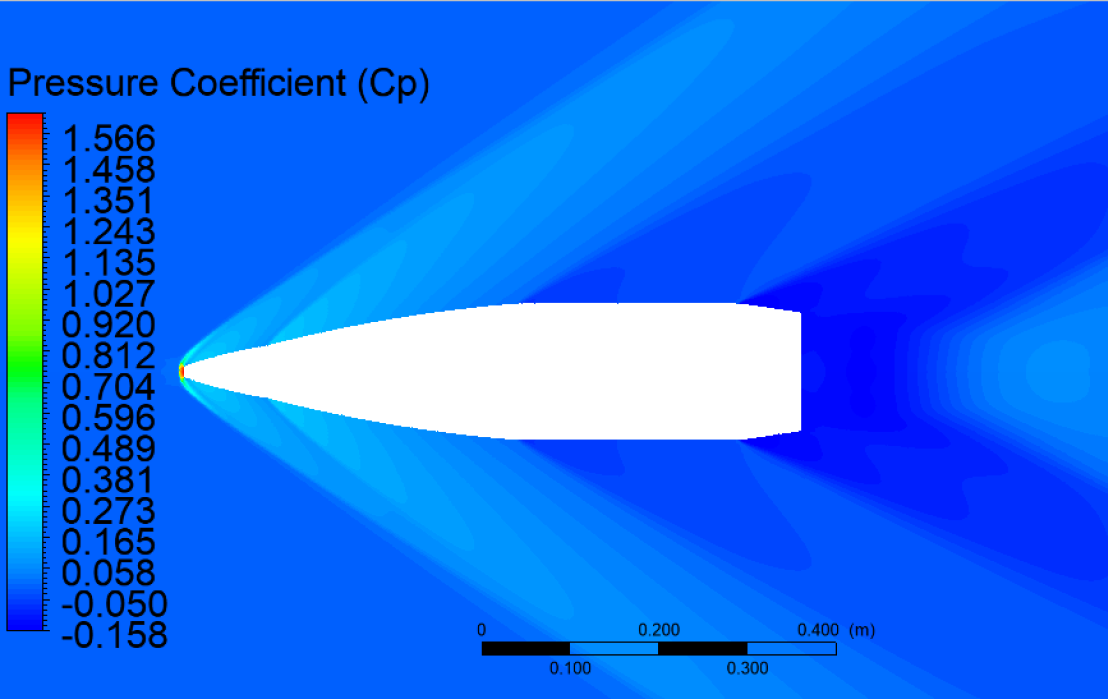
\includegraphics[height=5cm,width=\textwidth]{contorno-pressao-2306K-vazao-0030-2pol.png}
        \caption{Contornos de Pressão - \(\Dot{m}_{BB}\) = \qty{0,030}{\kilogram\per\second}}
        \label{fig:contorno-pressao-bb-2pol-vazao-0030}
    \end{subfigure}
    \hfill
    \begin{subfigure}[b]{0.47\textwidth}
        \centering
        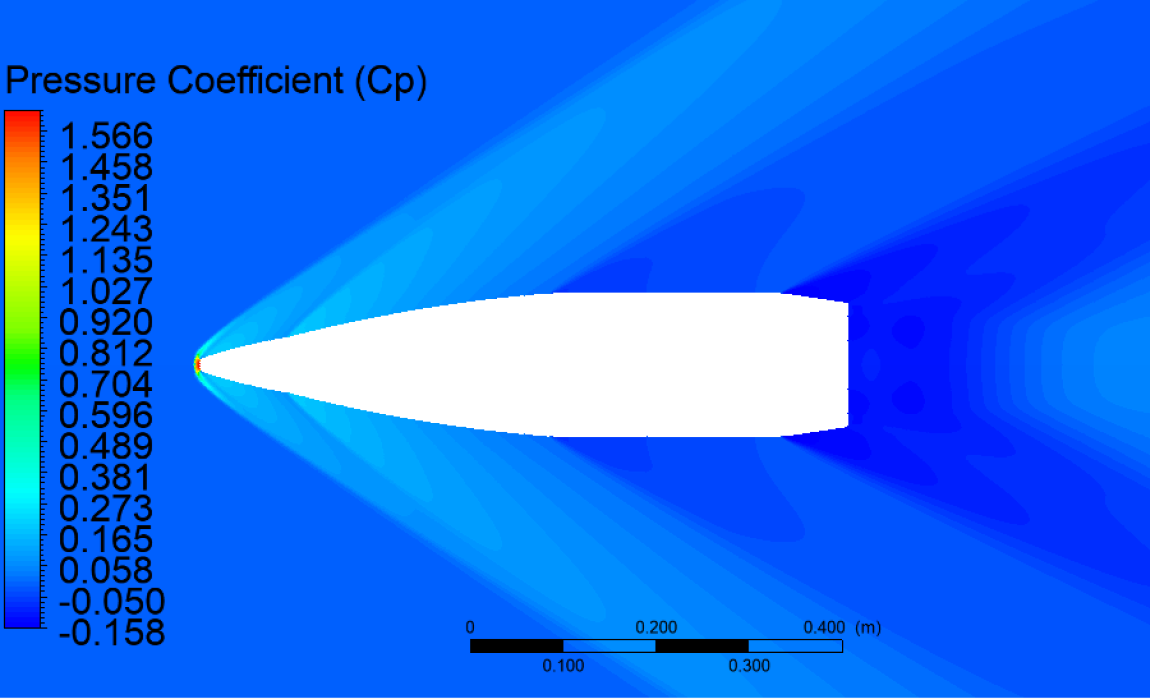
\includegraphics[height=5cm,width=\textwidth]{contorno-pressao-2306K-vazao-0060-2pol.png}
        \caption{Contornos de Pressão - \(\Dot{m}_{BB}\) = \qty{0,060}{\kilogram\per\second}}
        \label{fig:contorno-pressao-bb-2pol-vazao-0060}
    \end{subfigure}
    \hfill
    \begin{subfigure}[b]{0.47\textwidth}
        \centering
        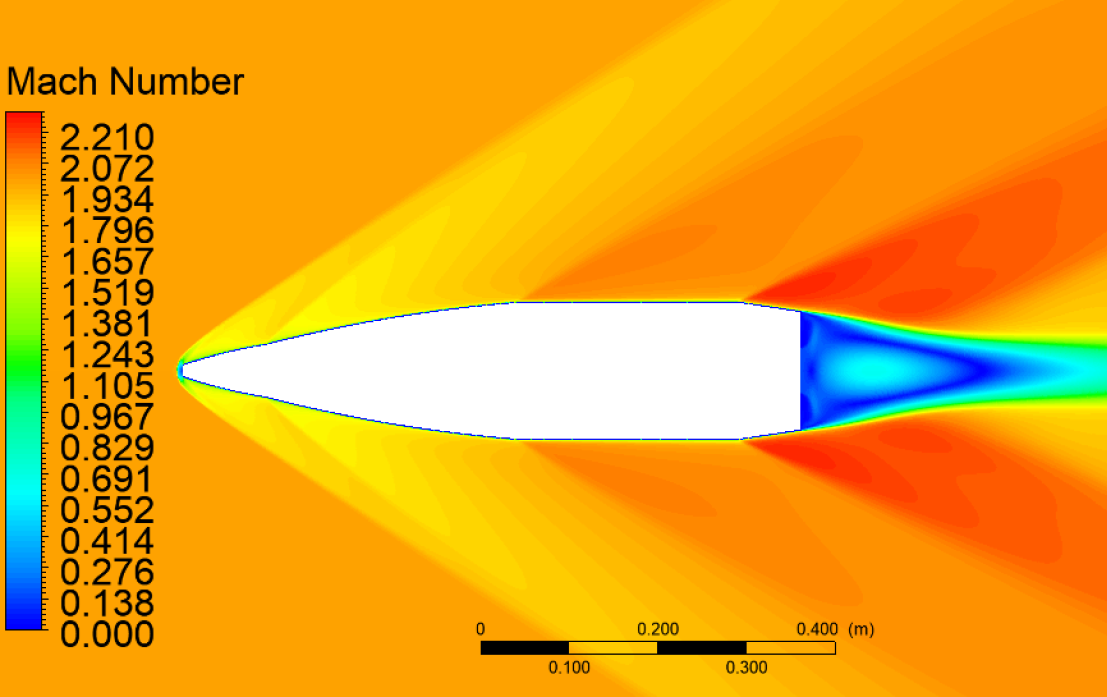
\includegraphics[height=5cm,width=\textwidth]{contorno-velocidade-2306K-vazao-0030-2pol.png}
        \caption{Cont. de Velocidade - \(\Dot{m}_{BB}\) = \qty{0,030}{\kilogram\per\second}}
        \label{fig:contorno-velocidade-bb-2pol-vazao-0030}
    \end{subfigure}
    \hfill
	\begin{subfigure}[b]{0.47\textwidth}
        \centering
        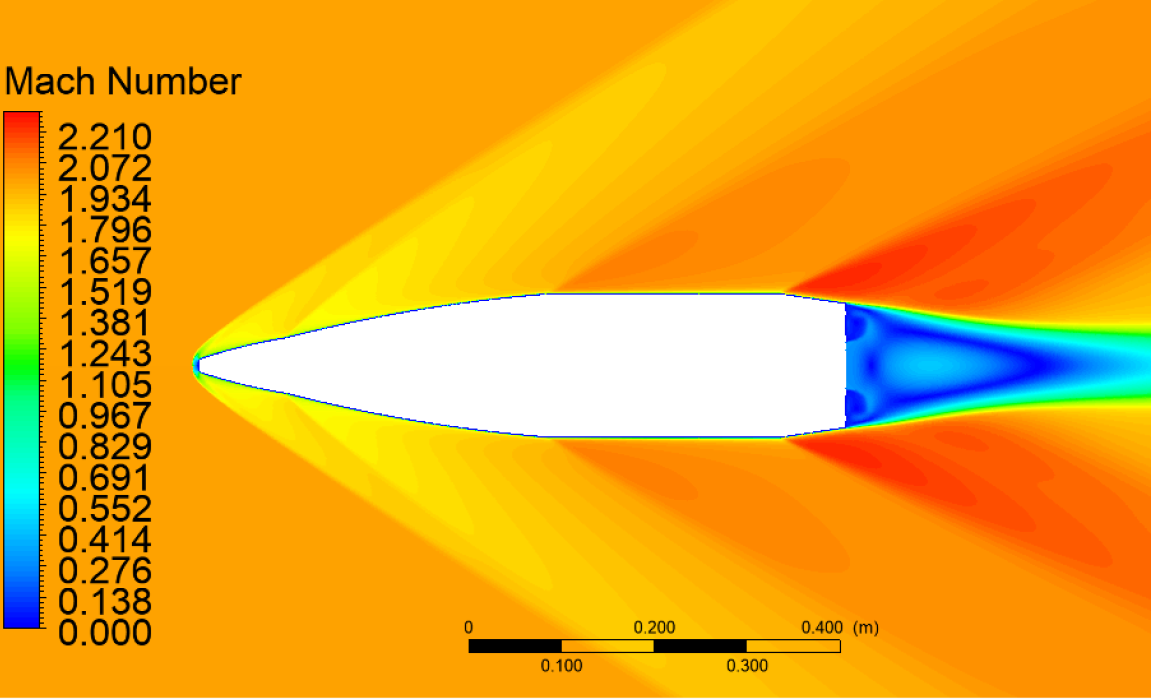
\includegraphics[height=5cm,width=\textwidth]{contorno-velocidade-2306K-vazao-0060-2pol.png}
        \caption{Cont. de Velocidade - \(\Dot{m}_{BB}\) = \qty{0,060}{\kilogram\per\second}}
        \label{fig:contorno-velocidade-bb-2pol-vazao-0060}
    \end{subfigure}
	\hfill
	\begin{subfigure}[b]{0.47\textwidth}
        \centering
        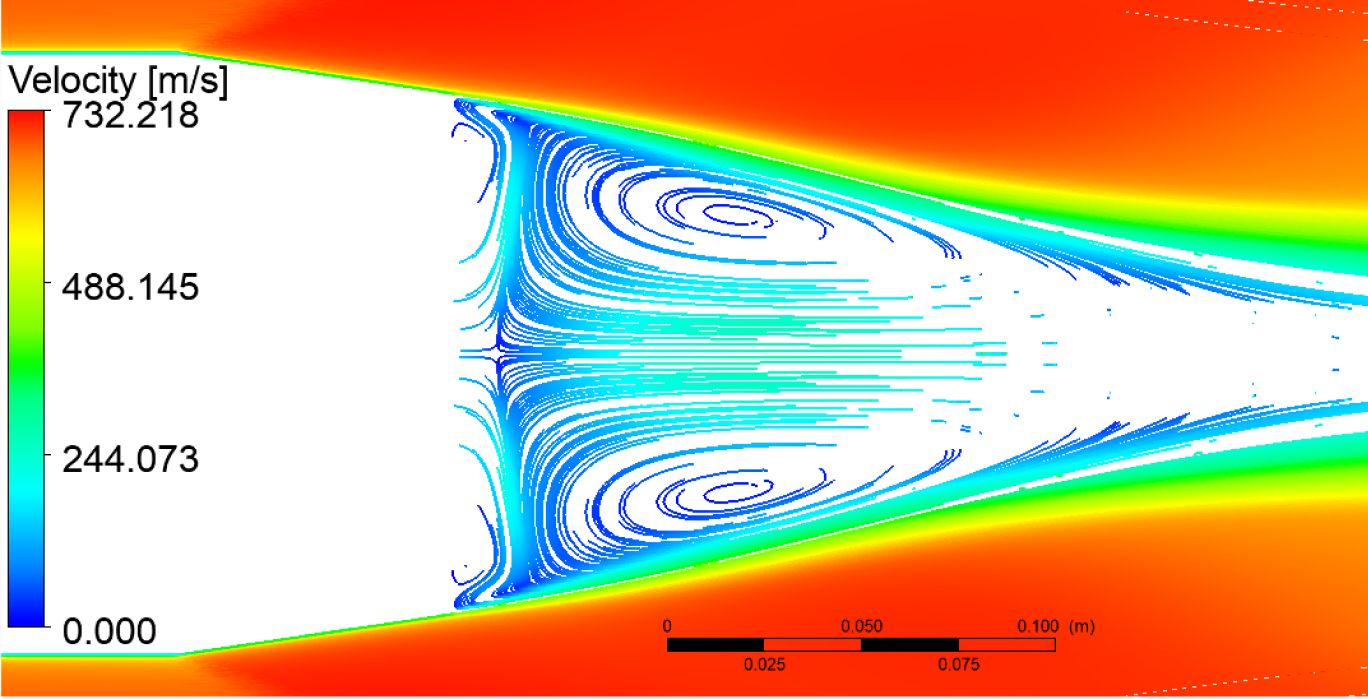
\includegraphics[height=5cm,width=\textwidth]{corrente-velocidade-2306K-vazao-0030-2pol.png}
        \caption{Linhas de Corrente - \(\Dot{m}_{BB}\) = \qty{0,030}{\kilogram\per\second}}
        \label{fig:corrente-velocidade-bb-2pol-vazao-0030}
    \end{subfigure}
    \hfill
    \begin{subfigure}[b]{0.47\textwidth}
        \centering
        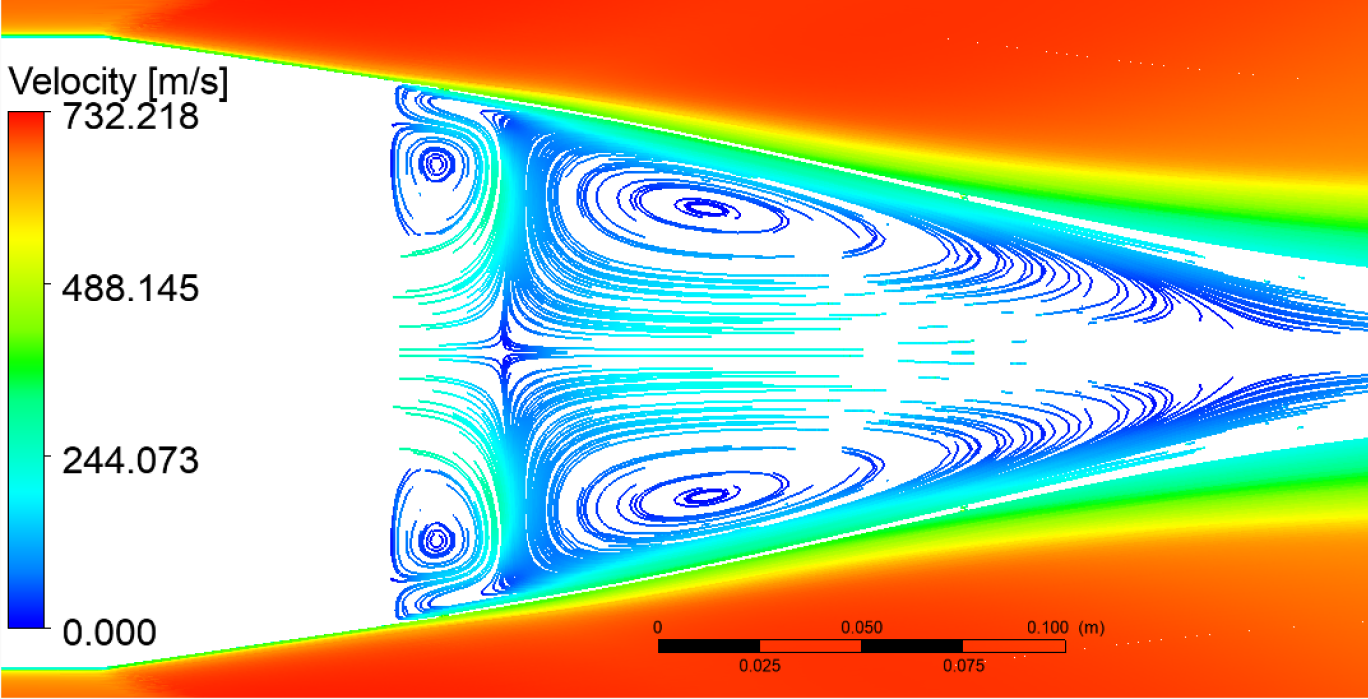
\includegraphics[height=5cm,width=\textwidth]{corrente-velocidade-2306K-vazao-0060-2pol.png}
        \caption{Linhas de Corrente - \(\Dot{m}_{BB}\) = \qty{0,060}{\kilogram\per\second}}
	\label{fig:corrente-velocidade-bb-2pol-vazao-0060}
    \end{subfigure}
	\caption{Projetil sob diferentes condições de vazão mássica sob regime M = \num{2,0} \(\left(\phi_{BB} = \qty{50,8}{\millimetre}; T_{BB} = \qty{2306,15}{\kelvin}\right)\)}
	\label{fig:influencia-diametro-vazao-2pol}
\end{figure}

\subsection{Influência da vazão mássica no sistema \textit{Base Bleed}} \label{subsec:resultados-com-basebleed-vazao}

A \autoref{fig:comparacao-basebleed-vazao} demonstra a influência da vazão nos resultados obtidos nas simulações computacionais com o efeito \textit{Base Bleed} na base do projetil, assumindo que a temperatura de saída dos gases foi fixada em \qty{1500}{\kelvin} e o diâmetro de saída do \textit{Base Bleed} escolhido foi de \qty{2}{\polegada} \(\left(\phi_{BB} = \qty{50,8}{\millimetre}\right)\). A escolha por esse diâmetro de saída se deve aos melhores resultados produzidos na \autoref{subsec:resultados-com-basebleed-diametros}.

Acerca do coeficiente de arrasto, nota-se na \autoref{fig:comparacao-basebleed-vazao} uma redução dos valores conforme aumenta a vazão mássica, \(\Dot{m}_{BB}\). As oscilações nos valores continuam aparecendo no regime subsônico, apesar de seguirem a mesma tendência, não importando qual vazão seja. O regime transônico reúne as maiores reduções do arrasto aerodinâmico, mas a redução do arrasto se faz menos efeito conforme aumenta a velocidade, passando pelo supersônico, especialmente quando M > \num{2,0}.

\begin{figure}[!ht]
	\centering
	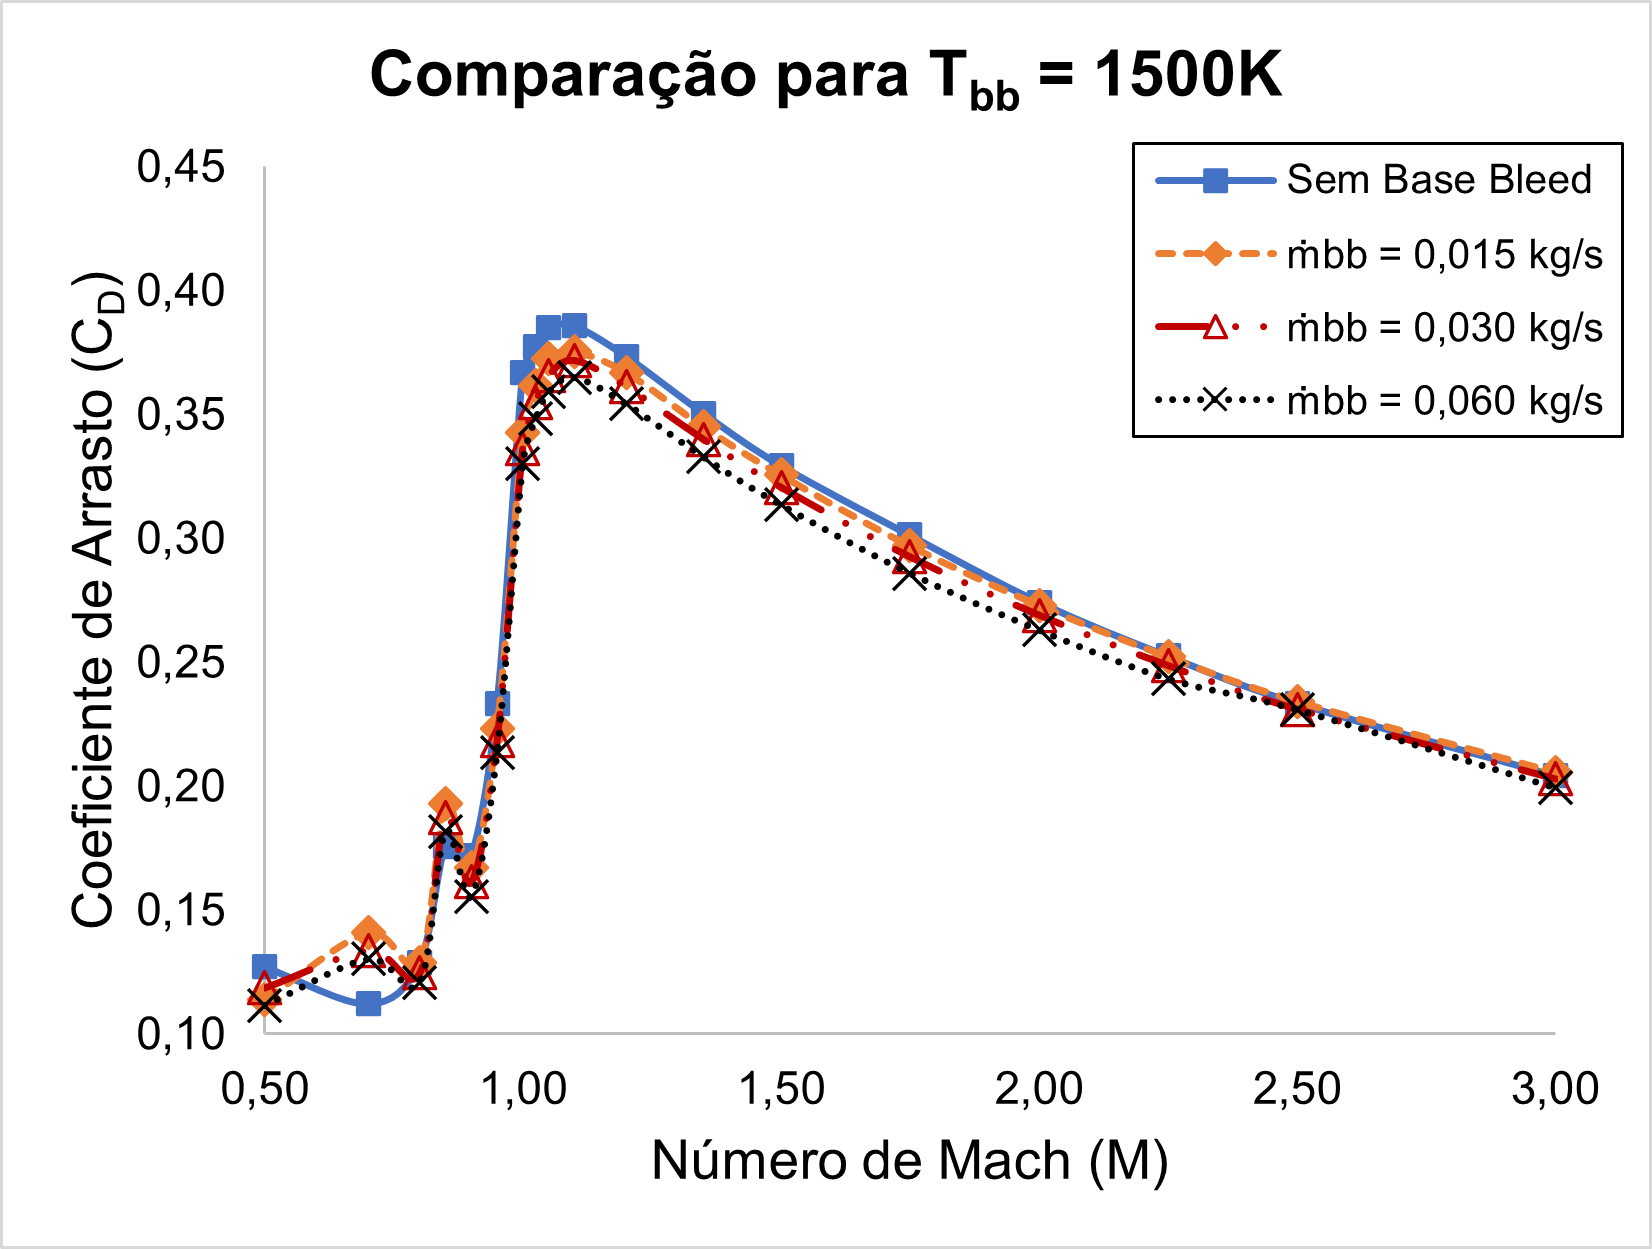
\includegraphics[width=0.5\textwidth]{cd-combasebleed-1500K-2pol.png}
	\caption{Influência da vazão mássica do \textit{Base Bleed} - \(T_{BB}\) = \qty{1500}{\kelvin}}
	\label{fig:comparacao-basebleed-vazao}
\end{figure}

\begin{figure}[!ht]
	\centering
	\begin{subfigure}[b]{0.47\textwidth}
        \centering
        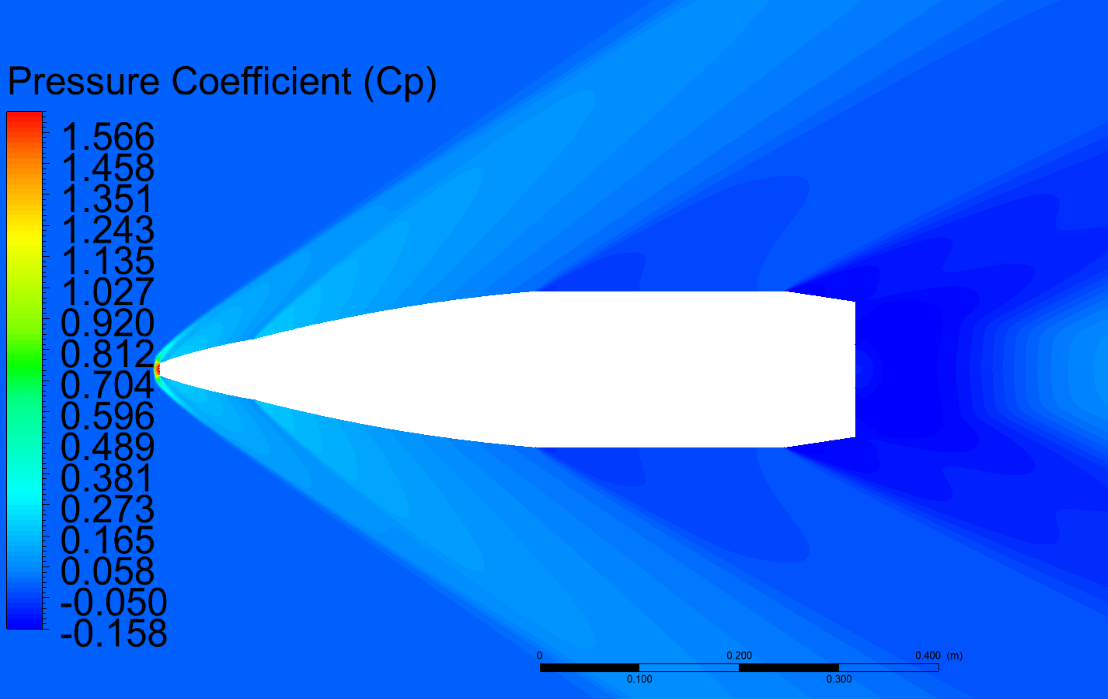
\includegraphics[width=\textwidth,height=5cm]{contorno-pressao-1500K-vazao-0030-2pol.png}
        \caption{Contornos de Pressão - \(\Dot{m}_{BB}\) = \qty{0,060}{\kilogram\per\second}}
        \label{fig:contorno-pressao-bb-1500K-vazao0030}
    \end{subfigure}
    \hfill
    \begin{subfigure}[b]{0.47\textwidth}
        \centering
        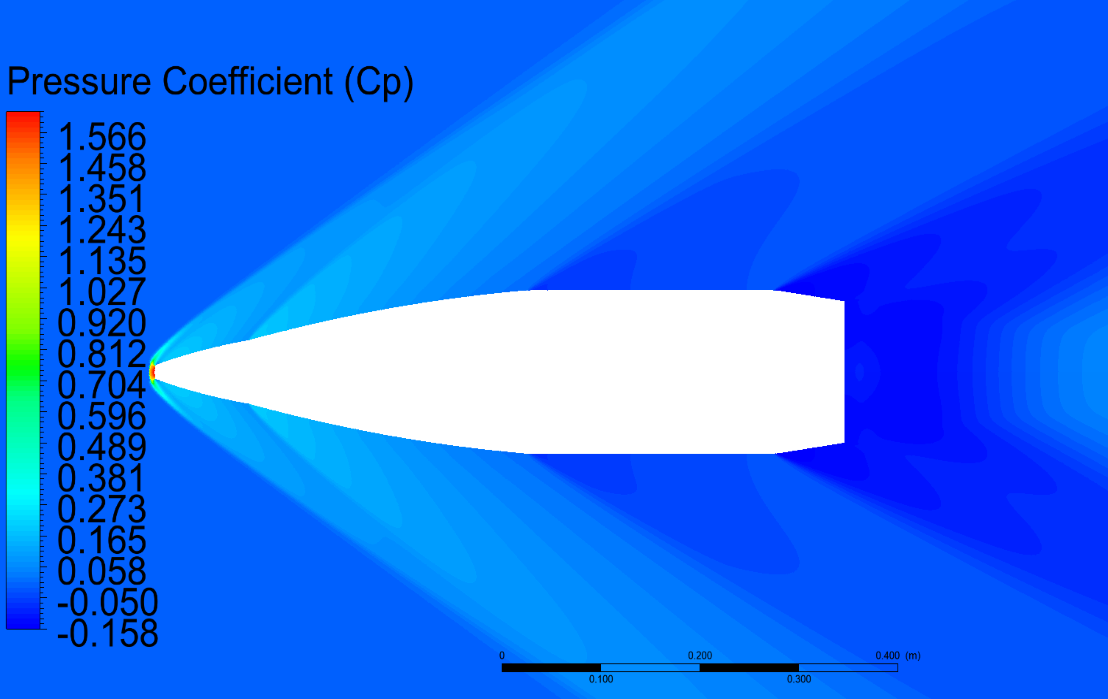
\includegraphics[width=\textwidth,height=5cm]{contorno-pressao-1500K-vazao-0060-2pol.png}
        \caption{Contornos de Pressão - \(\Dot{m}_{BB}\) = \qty{0,060}{\kilogram\per\second}}
        \label{fig:contorno-pressao-bb-1500K-vazao0060}
    \end{subfigure}
    \hfill
	\begin{subfigure}[b]{0.47\textwidth}
        \centering
        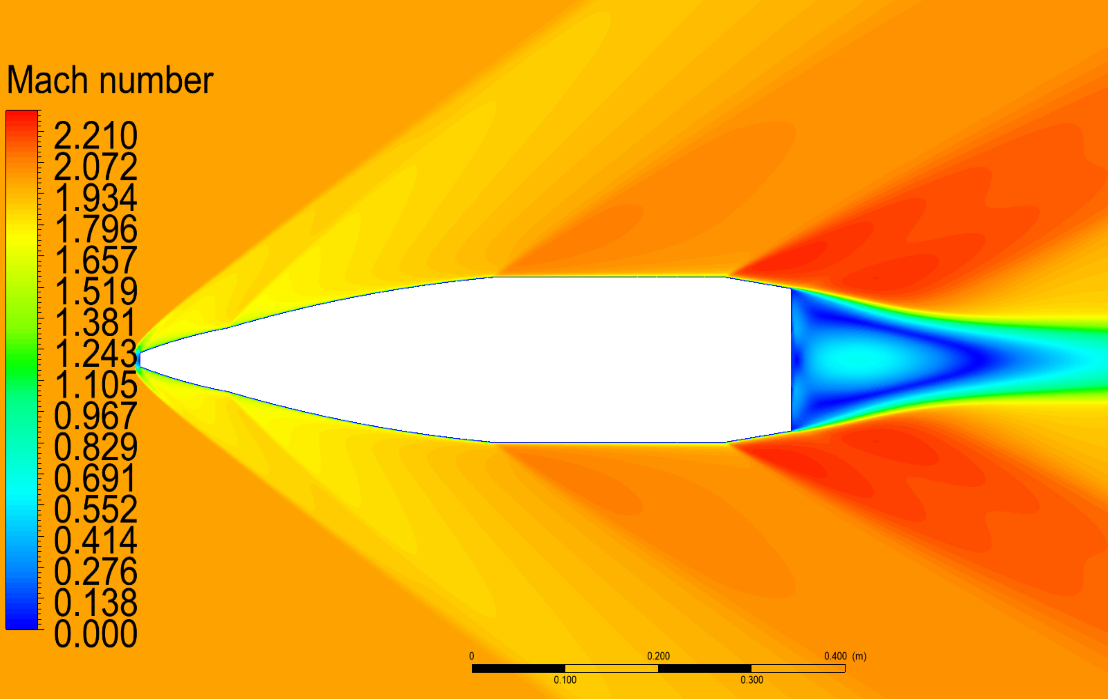
\includegraphics[width=\textwidth,height=5cm]{contorno-velocidade-1500K-vazao-0030-2pol.png}
        \caption{Cont. de Velocidade - \(\Dot{m}_{BB}\) = \qty{0,060}{\kilogram\per\second}}
        \label{fig:contorno-velocidade-bb-1500K-vazao0030}
    \end{subfigure}
    \hfill
	\begin{subfigure}[b]{0.47\textwidth}
        \centering
        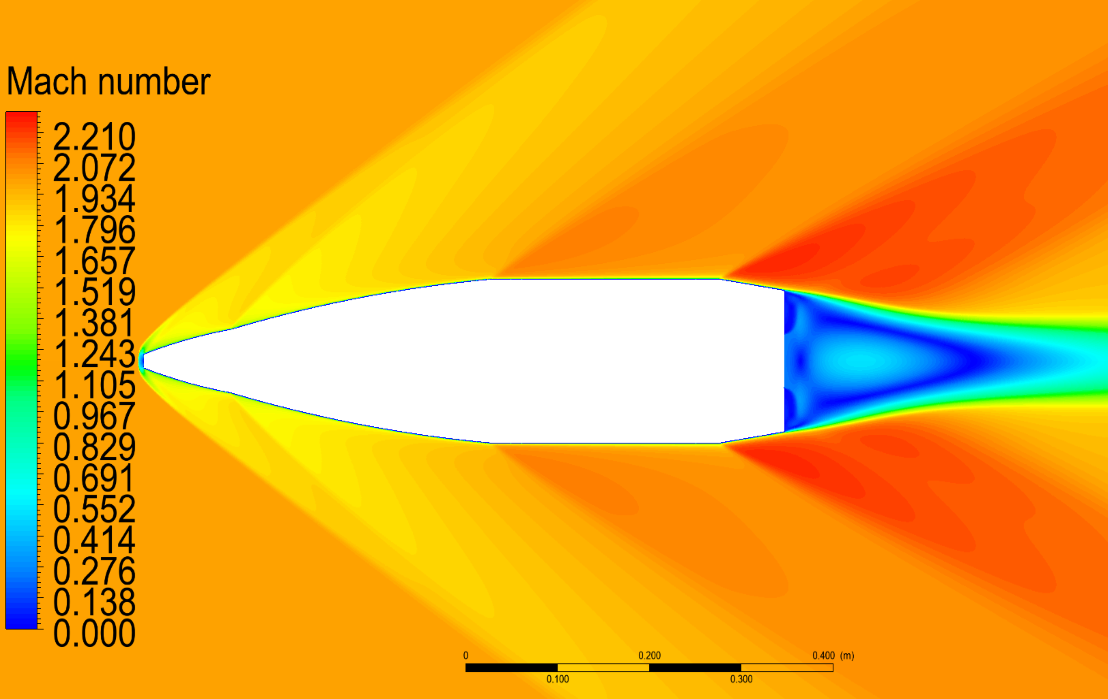
\includegraphics[width=\textwidth,height=5cm]{contorno-velocidade-1500K-vazao-0060-2pol.png}
        \caption{Cont. de Velocidade - \(\Dot{m}_{BB}\) = \qty{0,060}{\kilogram\per\second}}
        \label{fig:contorno-velocidade-bb-1500K-vazao0060}
    \end{subfigure}
    \begin{subfigure}[b]{0.47\textwidth}
        \centering
        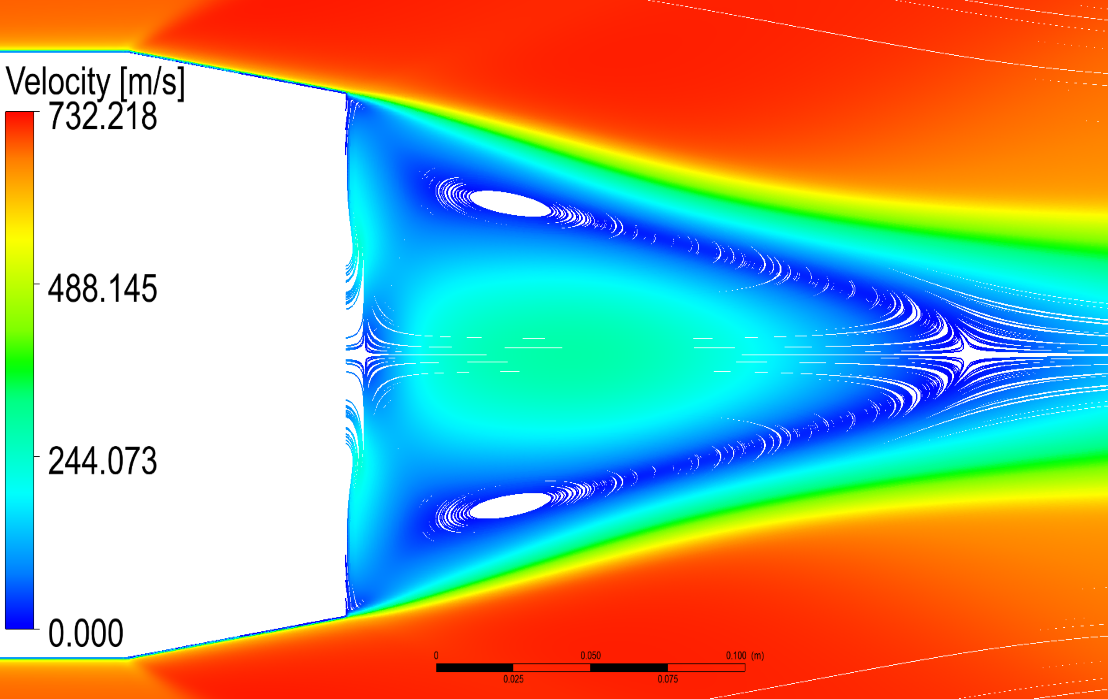
\includegraphics[width=\textwidth,height=5cm]{corrente-velocidade-1500K-vazao-0030-2pol.png}
        \caption{Linhas de Corrente - \(\Dot{m}_{BB}\) = \qty{0,060}{\kilogram\per\second}}
        \label{fig:corrente-velocidade-bb-1500K-vazao0030}
    \end{subfigure}
    \hfill
	\begin{subfigure}[b]{0.47\textwidth}
        \centering
        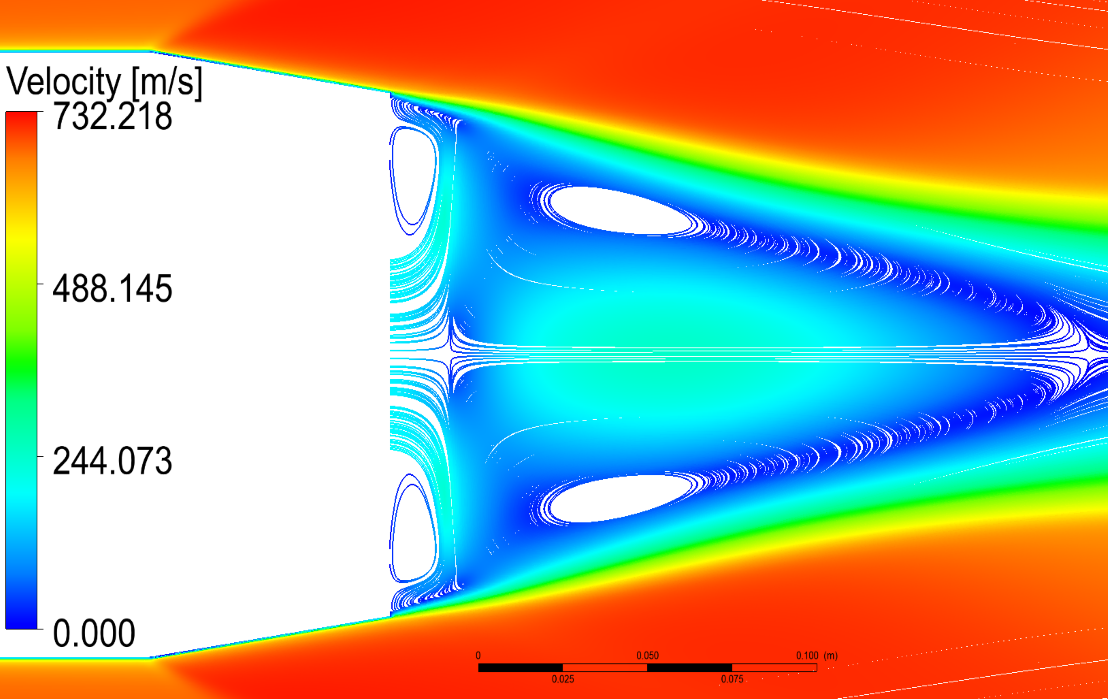
\includegraphics[width=\textwidth,height=5cm]{corrente-velocidade-1500K-vazao-0060-2pol.png}
        \caption{Linhas de Corrente - \(\Dot{m}_{BB}\) = \qty{0,060}{\kilogram\per\second}}
        \label{fig:corrente-velocidade-bb-1500K-vazao0060}
    \end{subfigure}
    \caption{Projetil sob diferentes condições de vazão mássica sob regime M = \num{2,0} \(\left(\phi_{BB} = \qty{50,8}{\millimetre}; T_{BB} = \qty{1500}{\kelvin}\right)\)}
	\label{fig:influencia-temperatura-bb}
\end{figure}

Conforme aumenta a vazão, há um aumento de velocidade, apesar de não haver acréscimo de pressão, o que é demonstrado pela \autoref{fig:contorno-pressao-bb-1500K-vazao0030} ou \autoref{fig:contorno-pressao-bb-1500K-vazao0060}. Os contornos de velocidade, presentes nas Figuras \ref{fig:contorno-velocidade-bb-1500K-vazao0030} e \ref{fig:contorno-velocidade-bb-1500K-vazao0060}, apresentam o deslocamento da região primária de recirculação, além do aumento da esteira turbulenta. 

Pelas Figuras \ref{fig:corrente-velocidade-bb-1500K-vazao0030} e \ref{fig:corrente-velocidade-bb-1500K-vazao0060} se observam as linhas de corrente para a velocidade. Em ambos os casos há a formação da recirculação anular, mas essa zona secundária de recirculação é mais proeminente conforme o aumento da vazão. A \autoref{fig:corrente-velocidade-bb-1500K-vazao0060} apresenta com maior clareza um valor mais próximo do que se espera ocorrer na região, dentro do que a literatura demonstrou em trabalhos anteriores \cite{Sahu1985,Andersson1976}. Assume-se que todos os contornos da \autoref{fig:influencia-temperatura-bb} estão sob regime M = \num{2,0}.

\subsection{Influência da temperatura}

A \autoref{fig:comparacao-basebleed-temperatura} demonstra a influência da temperatura nos resultados obtidos nas simulações computacionais com o efeito \textit{Base Bleed} na base do projetil, assumindo que a vazão mássica de saída dos gases foi fixada em \qty{0,060}{\kilogram\per\second} e o diâmetro de saída do \textit{Base Bleed} escolhido foi de \qty{2}{\polegada} \(\left(\phi_{BB} = \qty{50,8}{\millimetre}\right)\). A escolha por esse diâmetro de saída se deve aos melhores resultados produzidos na \autoref{subsec:resultados-com-basebleed-diametros}. A escolha pela vazão de \qty{0,060}{\kilogram\per\second} se baseou nos resultados das \autoref{subsec:resultados-com-basebleed-vazao}, em que a redução do coeficiente de arrasto foi mais significativo quando comparado ao projetil inerte.

\begin{figure}[!ht]
	\centering
	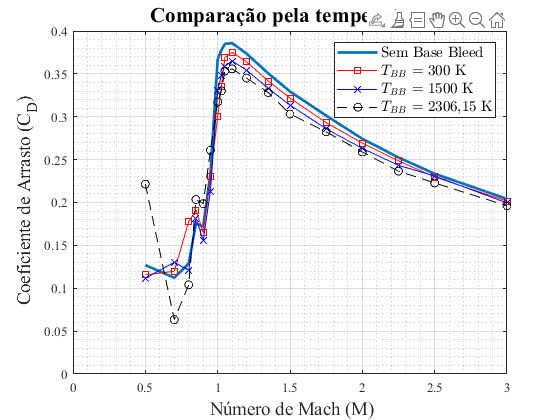
\includegraphics[width=0.5\textwidth]{cd-combasebleed-vazao006-2pol.png}
	\caption{Influência da temperatura do \textit{Base Bleed} sobre o coeficiente de arrasto com \(\Dot{m}_{BB}\) = \qty{0,060}{\kilogram\per\second}}
	\label{fig:comparacao-basebleed-temperatura}
\end{figure}

Acerca do coeficiente de arrasto, nota-se na \autoref{fig:comparacao-basebleed-temperatura} uma redução dos valores conforme aumenta a temperatura, \(Dot{m}_{BB}\). As oscilações nos valores continuam aparecendo no regime subsônico, embora tenham valores discrepantes no início da curva no caso em que a temperatura é mais elevada \(T_{BB} = \qty{2306,15}{\kelvin}\). Mesmo assim, seguem a mesma tendência, não importando qual vazão seja. O regime transônico reúne as maiores reduções do arrasto aerodinâmico, mas a redução do arrasto também é considerável no regime supersônico, principalmente o valor de Mach entre \numrange{1,5}{2,0}. Após esse intervalo, a redução é mais gradual.

\subsection{Influência da abordagem RANS}\label{subsec:resultados-com-basebleed-RANS}

Conforme foi citado anteriormente, o modelo Spalart-Allmaras \cite{Spalart1992} foi manejado para atestar a eficiência de outra técnica RANS para descrição da turbulência além do que foi proposto por \citeauthor{Menter1994TwoequationET}. A comparação foi realizada somente para os seguintes valores na condição de contorno \textit{base bleed inlet}: \(\Dot{m}_{BB}\) = \qty{50,8}{\millimetre}, \(T_{BB} = \qty{2306,15}{\kelvin}\) e \(\Dot{m}_{BB}\) = \qty{0,060}{\kilogram\per\second}.

Entretanto, é notório que o modelo Spalart-Allmaras (S-A) superestimou a curva de arrasto em todos os regimes de velocidade, relatado pela Figura \ref{fig:comparacao-bb-rans}.

\begin{figure}[!ht]
    \centering
    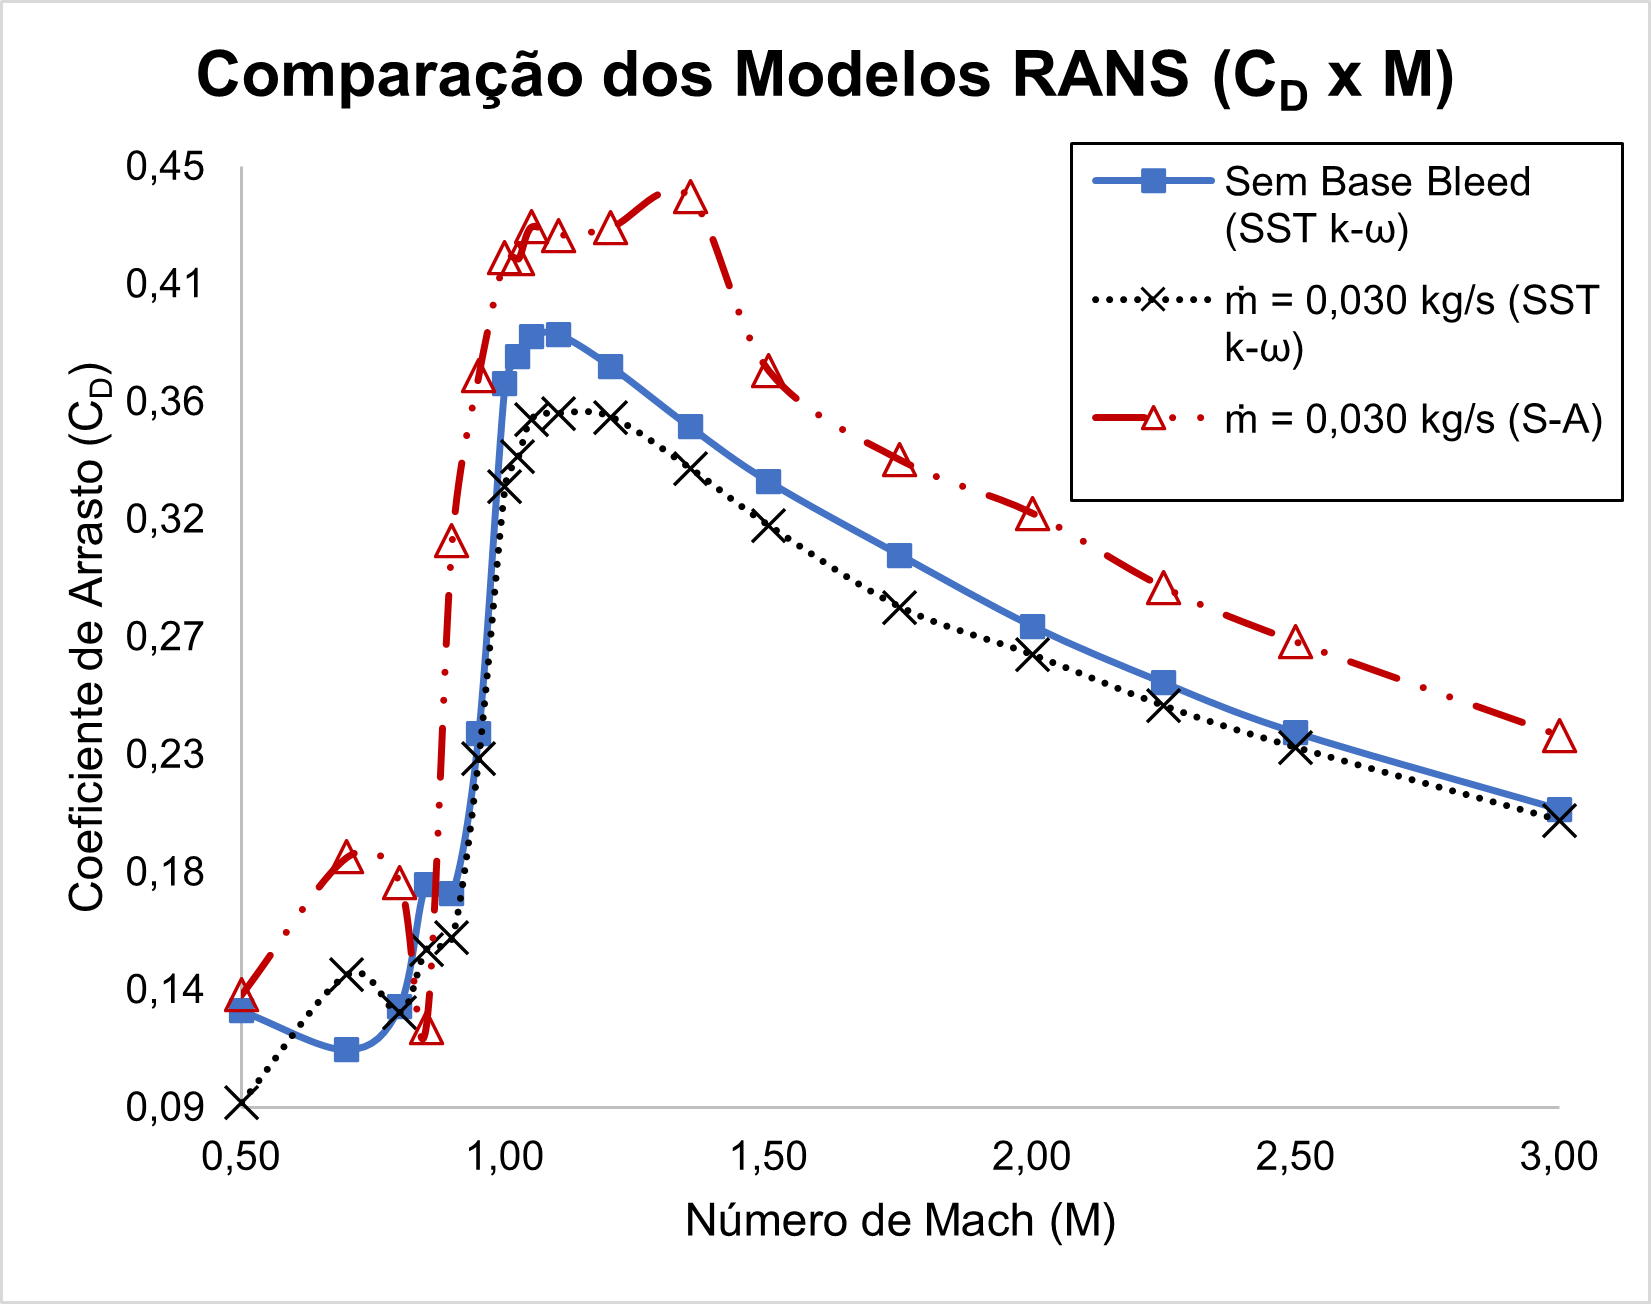
\includegraphics[width=0.5\textwidth]{cd-combasebleed-rans.png}
 	\caption{Curvas de arrasto de acordo com modelos de turbulência RANS}
    \label{fig:comparacao-bb-rans}
\end{figure}

De acordo com a apresentação da \autoref{fig:contornos-pressao-velocidade-RANS}, o modelo S-A não conseguiu encontrar a zona de recirculação gerada pelo sistema \textit{base bleed} como tampouco registra o momento provocado pela vazão mássica de gases do propelente.

\begin{figure}[!ht]
	\centering
	\begin{subfigure}[b]{0.47\textwidth}
        \centering
        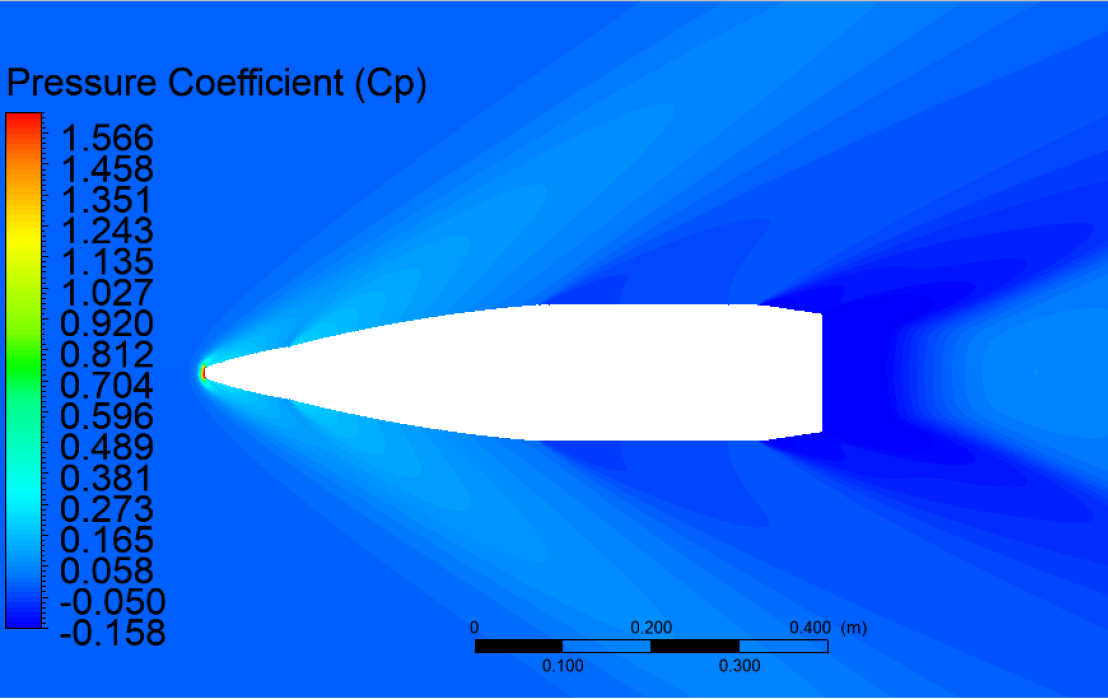
\includegraphics[height=5cm,width=\textwidth]{contorno-pressao-SPALART-2pol.png}
        \caption{Contornos de Pressão}
        \label{fig:contorno-pressao-bb-2pol-RANS}
    \end{subfigure}
    \hfill
    \begin{subfigure}[b]{0.47\textwidth}
        \centering
        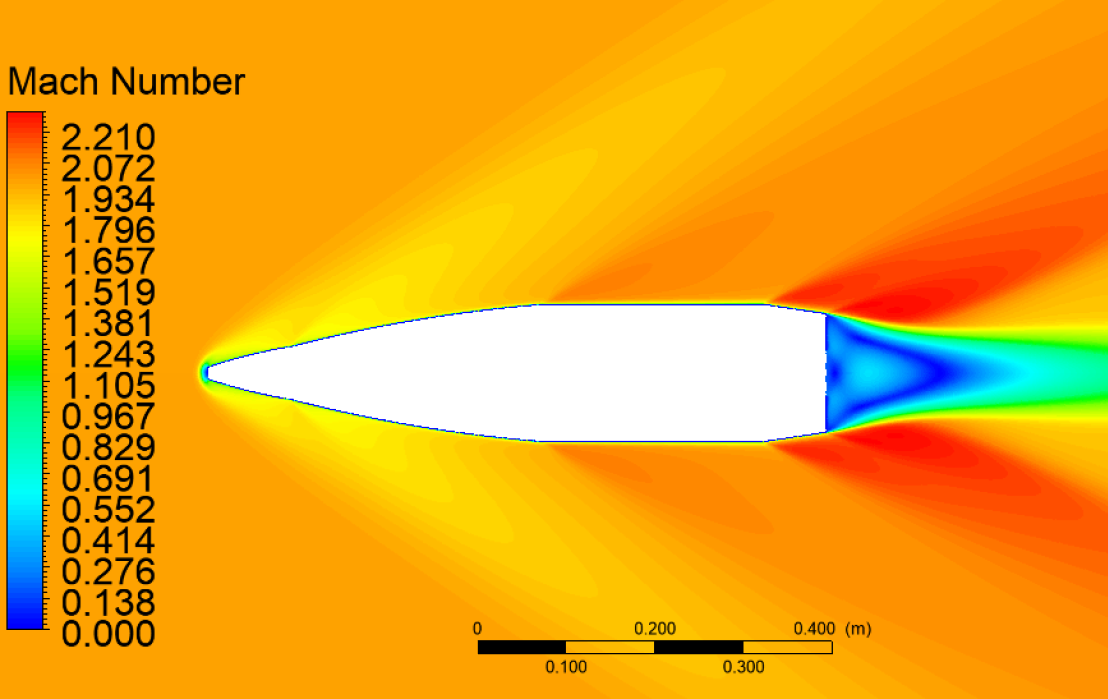
\includegraphics[height=5cm,width=\textwidth]{contorno-velocidade-SPALART-2pol.png}
        \caption{Contornos de Velocidade}
        \label{fig:contorno-velocidade-bb-2pol-RANS}
    \end{subfigure}
	\caption{Projetil sob modelo Spalart-Allmaras}
	\label{fig:contornos-pressao-velocidade-RANS}
\end{figure}

Para assegurar o que foi demonstrado na \autoref{fig:contorno-pressao-bb-2pol-RANS}, a \autoref{fig:corrente-velocidade-bb-RANS} foi elaborada para analisar as linhas de corrente com o modelo de 1 equação, donde se concluiu que o alto gradiente adverso de pressão existente no sistema BB resultou em desvios que fogem da explicação do fenômeno físico real, ainda que as técnicas RANS enxerguem os valores médios das propriedades do fluido.

\begin{figure}[!ht]
    \centering
    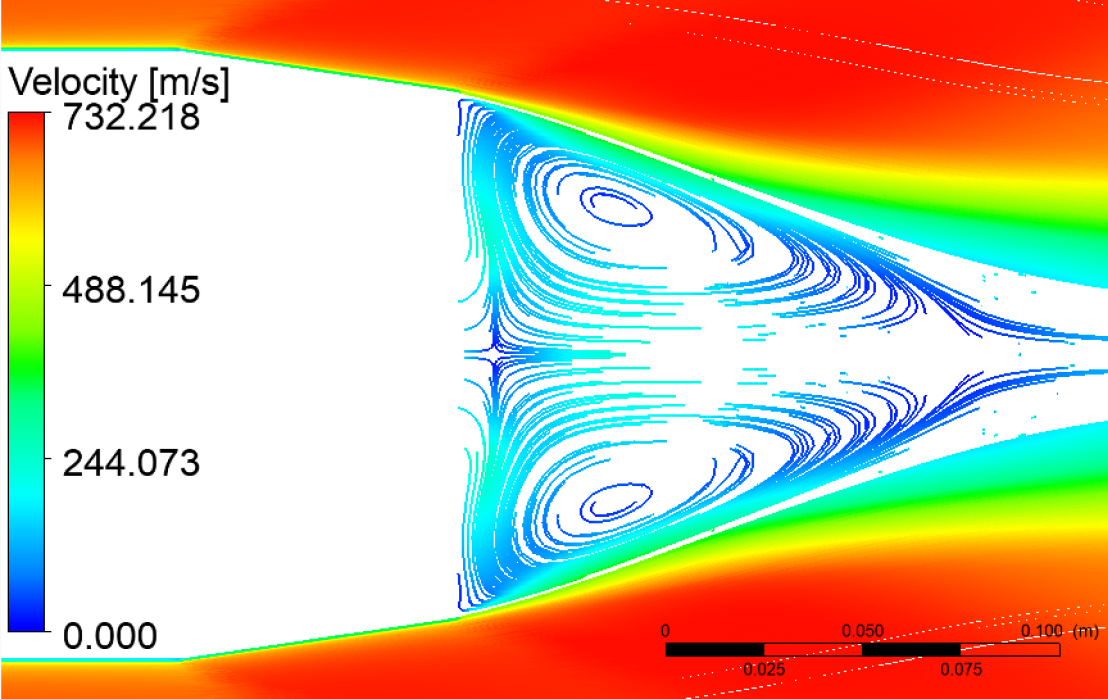
\includegraphics[height=5cm,width=0.5\textwidth]{corrente-velocidade-SPALART-2pol.png}
 	\caption{Linhas de corrente para o modelo Spalart-Allmaras}
    \label{fig:corrente-velocidade-bb-RANS}
\end{figure}

\section{Resultados da Trajetória}\label{sec:resultados-trajetoria}

A partir do momento em que há disponibilidade das condições citadas na \autoref{subsec:implementacao-trajetoria} e dos resultados das simulações de fluidodinâmica computacional, pode-se calcular a predição da trajetória MPMTM. Apesar do suporte do PRODAS® e das informações obtidas, algumas premissas foram consideradas:

\begin{itemize}
    \item Lançamento do Rio de Janeiro, logo a latitude é de \ang{23};
    \item Desprezando efeitos da umidade sobre a atmosfera;
    \item Sem velocidade do vento, assim como citado por \citeauthor{Rosendo2020};
    \item Vazão mássica do propelente é constante durante o acionamento do BB;
    \item Parâmetro ótimo de injeção \(\left(Inj_{0}\right)\) igual a \num{5e-3}, tal como descrito por \citeauthor{DAVENAS1993329};
    \item Assumir que os coeficientes aerodinâmicos são linearmente dependentes do ângulo \(\alpha_{e}\)
\end{itemize}

Pela última condição assumida, logo \(C_{L\alpha^{3}}\) e \(C_{m\alpha^{3}}\) não interferem significativamente as equações \ref{eq:liftMPM} e \ref{eq:guinada-de-reposicao}. Embora a ignição seja um tópico relevante no desempenho, a dificuldade em modelar adequadamente à realidade tornou o assunto um caso a ser tratado em estudos posteriores.
De acordo com o STANAG 4355 \cite{stanag4355}, é necessário obter os fatores \(f_{L}\) e \(i_{BB}\) tais que se adequem à cada simulação realizada. 

Para averiguar a qualidade do código desenvolvido em MATLAB®, os resultados obtidos de acordo com as condições de um projetil \qty{155}{\millimetre} a velocidade de disparo v = \qty{207,3}{\metre\per\second} foram analisadas tanto em função do PRODAS® quanto para uma tabela de tiro. Como pode ser visto na \autoref{tab:tabela-validacao-PRODAS-e-tabela-de-tiro-M107} \cite{Thallyo2022}, os erros foram superiores a \qty{1}{\percent} somente para trajetórias de grandes elevações, em que a literatura prevê inconsistências \cite{McCoy2012,Carlucci2018}.

\begin{table}[ht]
    \centering
    \caption[Resultados obtidos durante a validação (munição \qty{155}{\millimetre} M107)]{Resultados obtidos durante a validação (munição \qty{155}{\millimetre} M107)}
    \vspace{0.5cm}
    \resizebox{\textwidth}{!}{%
    \begin{tabular}{c|c|c|c|c|c|c|c}
    \hline
    \multicolumn{4}{c|}{PRODAS®} &
      \multicolumn{4}{c}{Tabela de tiro} \\ \hline
    \multicolumn{1}{c|}{\multirow{2}{*}{\begin{tabular}[c]{@{}c@{}}Elevação \\ (\unit{\milliradian})\end{tabular}}} &
      \multicolumn{2}{c|}{Alcance (\unit{\metre})} &
      \multirow{2}{*}{\begin{tabular}[c]{@{}c@{}}Erro \\ (\unit{\percent})\end{tabular}} &
      \multicolumn{1}{c|}{\multirow{2}{*}{\begin{tabular}[c]{@{}c@{}}Elevação \\ (\unit{\milliradian})\end{tabular}}} &
      \multicolumn{2}{c|}{Alcance (\unit{\metre})} &
      \multirow{2}{*}{\begin{tabular}[c]{@{}c@{}}Erro \\ (\unit{\percent})\end{tabular}} \\ \cline{2-3} \cline{6-7}
    \multicolumn{1}{c|}{} &
      \multicolumn{1}{c|}{Esperado} &
      \multicolumn{1}{c|}{Obtido} &
       &
      \multicolumn{1}{c|}{} &
      \multicolumn{1}{c|}{Esperado} &
      \multicolumn{1}{c|}{Obtido} &
       \\ \hline
    \num{58,9} &
      \num{500,0} &
      \num{501,2} &
      \num{0,24} &
      \num{58,9} &
      \num{500,0} &
      \num{501,2} &
      \num{0,24} \\
    \num{120,1} &
      \num{1000,0} &
      \num{1001,9} &
      \num{0,19} &
      \num{120,3} &
      \num{1000,0} &
      \num{1003,5} &
      \num{0,35} \\
    \num{184,7} &
      \num{1500,0} &
      \num{1501,7} &
      \num{0,11} &
      \num{185,3} &
      \num{1500,0} &
      \num{1506,2} &
      \num{0,41} \\
    \num{254,5} &
      \num{2000,0} &
      \num{2001,7} &
      \num{0,09} &
      \num{255,4} &
      \num{2000,0} &
      \num{2007,9} &
      \num{0,40} \\
    \num{332,1} &
      \num{2500,0} &
      \num{2501,1} &
      \num{0,04} &
      \num{333,5} &
      \num{2500,0} &
      \num{2509,5} &
      \num{0,38} \\
    \num{422,9} &
      \num{3000,0} &
      \num{2999,9} &
      \num{0,00} &
      \num{424,7} &
      \num{3000,0} &
      \num{3008,8} &
      \num{0,29} \\
    \num{541,9} &
      \num{3500,0} &
      \num{3498,9} &
      \num{0,03} &
      \num{543,8} &
      \num{3500,0} &
      \num{3505,3} &
      \num{0,15} \\
    \num{731,3} &
      \num{3900,0} &
      \num{3897,6} &
      \num{0,06} &
      \num{729,2} &
      \num{3900,0} &
      \num{3896,0} &
      \num{0,11} \\
    \num{838,4} &
      \num{3900,0} &
      \num{3898,3} &
      \num{0,05} &
      \num{846,2} &
      \num{3900,0} &
      \num{3891,9} &
      \num{0,21} \\
    \num{1027,5} &
      \num{3500,0} &
      \num{3504,3} &
      \num{0,11} &
      \num{1028,3} &
      \num{3500,0} &
      \num{3501,5} &
      \num{0,03} \\
    \num{1144,7} &
      \num{3000,0} &
      \num{3016,7} &
      \num{0,53} &
      \num{1141,1} &
      \num{3000,0} &
      \num{3034,3} &
      \num{1,12} \\
    \num{1231,4} &
      \num{2500,0} &
      \num{2539,9} &
      \num{1,55} &
      \num{1220,5} &
      \num{2500,0} &
      \num{2605,5} &
      \num{4,18} \\ \hline
    \end{tabular}%
    }
    \label{tab:tabela-validacao-PRODAS-e-tabela-de-tiro-M107}
    \fonte{\cite{Thallyo2022}}
\end{table}

A metodologia para provar a eficiência do \textit{Base Bleed} foi demonstrar os alcances obtidos em simulações computacionais. A \autoref{fig:trajetoria-1pol-711mil} esclarece os resultados das predições de voo. A \autoref{tab:tabela-711mil-bb-1pol} mostra que houve redução do alcance e do apogeu.

\begin{figure}[!ht]
	\centering
    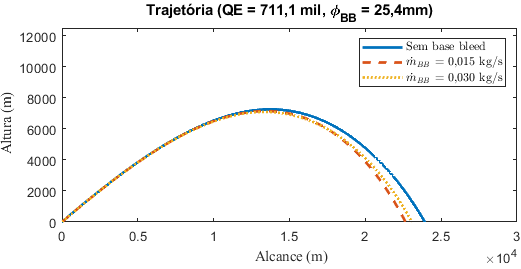
\includegraphics[width=0.7\textwidth]{foto1-qe711mil-1pol.png}
    \caption[QE = \qty{711}{\milliradian} \(\left(\phi_{BB} = \qty{25,4}{\millimetre}\right)\)]{QE = \qty{711}{\milliradian} \(\left(\phi_{BB} = \qty{25,4}{\millimetre}\right)\)}
    \label{fig:trajetoria-1pol-711mil}
\end{figure}

\begin{table}[ht]
\centering
\caption[Trajetória Balística com QE = \qty{711}{\milliradian} e v = \qty{878}{\metre\per\second} \(\left(\phi_{BB} = \qty{25,4}{\millimetre}\right)\)]{Trajetória Balística com QE = \qty{711}{\milliradian} e v = \qty{878}{\metre\per\second} \(\left(\phi_{BB} = \qty{25,4}{\millimetre}\right)\)}
\vspace{0.5cm}
\begin{tabular}{c|c|c|c|c}
Vazão Mássica & Alcance & Aumento & Apogeu & Aumento \\
\hline
\qty{0}{\kilogram\per\second} & \qty{23922,2}{\metre} & -- & \qty{7256,8}{\metre} & -- \\ 
\qty{0,015}{\kilogram\per\second} & \qty{22647,8}{\metre} & \qty{-5,3}{\percent} & \qty{7145,0}{\metre} & \qty{-1,5}{\percent} \\
\qty{0,030}{\kilogram\per\second} & \qty{23069,0}{\metre} & \qty{-3,6}{\percent} & \qty{7093,4}{\metre} & \qty{-2,3}{\percent}
\end{tabular}
\label{tab:tabela-711mil-bb-1pol}
\fonte{Autor.}
\end{table}

Acerca da \autoref{fig:trajetoria-1pol-800mil}, apesar de haver um aumento do alcance dos lançamentos sob efeito BB, os resultados também foram piores, quando comparados com o lançamento inerte. A \autoref{tab:tabela-800mil-bb-1pol} demonstra resultados percentuais muito próximos dos que foram apresentados na tabela anterior.

\begin{figure}[!ht]
	\centering
    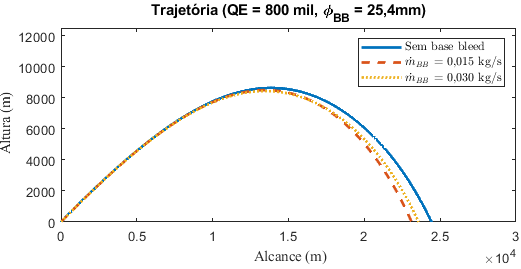
\includegraphics[width=0.7\textwidth]{foto2-qe800mil-1pol.png}
    \caption[QE = \qty{800}{\milliradian} \(\left(\phi_{BB} = \qty{25,4}{\millimetre}\right)\)]{QE = \qty{800}{\milliradian} \(\left(\phi_{BB} = \qty{25,4}{\millimetre}\right)\)}
    \label{fig:trajetoria-1pol-800mil}
\end{figure}

\begin{table}[ht]
\centering
\caption[Trajetória Balística com QE = \qty{800}{\milliradian} e v = \qty{878}{\metre\per\second} \(\left(\phi_{BB} = \qty{25,4}{\millimetre}\right)\)]{Trajetória Balística com QE = \qty{800}{\milliradian} e v = \qty{878}{\metre\per\second} \(\left(\phi_{BB} = \qty{25,4}{\millimetre}\right)\)}
\vspace{0.5cm}
\begin{tabular}{c|c|c|c|c}
Vazão Mássica & Alcance & Aumento & Apogeu & Aumento \\
\hline
\qty{0}{\kilogram\per\second} & \qty{24429,5}{\metre} & -- & \qty{8638,6}{\metre} & -- \\ 
\qty{0,015}{\kilogram\per\second} & \qty{23117,9}{\metre} & \qty{-5,4}{\percent} & \qty{8493,6}{\metre} & \qty{-1,7}{\percent} \\
\qty{0,030}{\kilogram\per\second} & \qty{23577,0}{\metre} & \qty{-3,5}{\percent} & \qty{8435,9}{\metre} & \qty{-2,3}{\percent}
\end{tabular}
\label{tab:tabela-800mil-bb-1pol}
\fonte{Autor.}
\end{table}

Ao verificar a \autoref{fig:trajetoria-2pol-711mil} percebe-se um aumento do alcance e do apogeu, atestado pela \autoref{tab:tabela-711mil-bb-2pol}. Há o aumento do alcance de quase \qty{6}{\percent} quando \(\Dot{m}_{BB} = \qty{0,060}{\kilogram\per\second}\).

\begin{figure}[!ht]
	\centering
    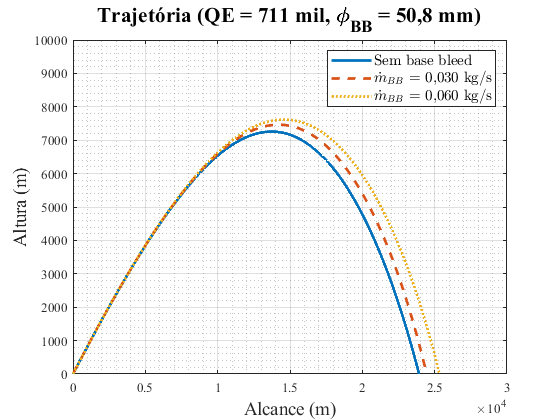
\includegraphics[width=0.7\textwidth]{foto3-qe711mil-2pol.png}
    \caption[QE = \qty{711}{\milliradian} \(\left(\phi_{BB} = \qty{50,8}{\millimetre}\right)\)]{QE = \qty{711}{\milliradian} \(\left(\phi_{BB} = \qty{50,8}{\millimetre}\right)\)}
    \label{fig:trajetoria-2pol-711mil}
\end{figure}

\begin{table}[!ht]
\centering
\caption[Trajetória Balística com QE = \qty{711}{\milliradian} e v = \qty{878}{\metre\per\second} \(\left(\phi_{BB} = \qty{50,8}{\millimetre}\right)\)]{Trajetória Balística com QE = \qty{711}{\milliradian} e v = \qty{878}{\metre\per\second} \(\left(\phi_{BB} = \qty{50,8}{\millimetre}\right)\)}
\vspace{0.5cm}
\begin{tabular}{c|c|c|c|c}
Vazão Mássica & Alcance & Aumento & Apogeu & Aumento \\
\hline
\qty{0}{\kilogram\per\second} & \qty{23922,2}{\metre} & -- & \qty{7256,8}{\metre} & -- \\
\qty{0,030}{\kilogram\per\second} & \qty{24439,8}{\metre} & \qty{2,2}{\percent} & \qty{7463,5}{\metre} & \qty{2,8}{\percent} \\
\qty{0,060}{\kilogram\per\second} & \qty{25334,3}{\metre} & \qty{5,9}{\percent} & \qty{7616,6}{\metre} & \qty{5,0}{\percent}
\end{tabular}
\label{tab:tabela-711mil-bb-2pol}
\fonte{Autor.}
\end{table}

Ao aumentar o ângulo de elevação para \qty{800}{\milliradian} houve um incremento percentual sobre o alcance e o apogeu também, como demonstrado na \autoref{fig:trajetoria-2pol-800mil}. Os resultados seguiram a mesma ordem de crescimento do deslocamento, quando se compara a \autoref{tab:tabela-711mil-bb-2pol} com a \autoref{tab:tabela-800mil-bb-2pol}. De qualquer forma, o diâmetro de saída do bocal tem forte influência na balística externa do projetil.

\begin{figure}[!ht]
	\centering
    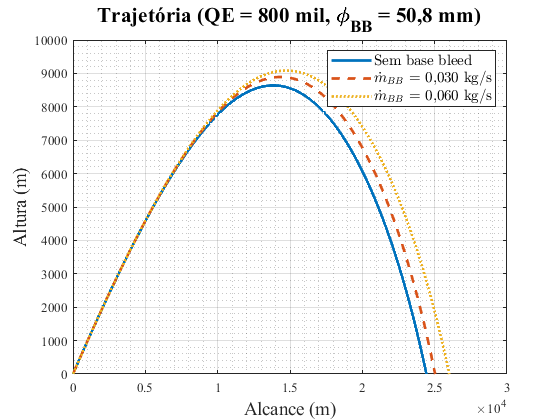
\includegraphics[width=0.7\textwidth]{foto4-qe800mil-2pol.png}
    \caption[QE = \qty{800}{\milliradian} \(\left(\phi_{BB} = \qty{50,8}{\millimetre}\right)\)]{QE = \qty{800}{\milliradian} \(\left(\phi_{BB} = \qty{50,8}{\millimetre}\right)\)}
    \label{fig:trajetoria-2pol-800mil}
\end{figure}

\begin{table}[ht]
\centering
\caption[Trajetória Balística com QE = \qty{800}{\milliradian} e v = \qty{878}{\metre\per\second} \(\left(\phi_{BB} = \qty{50,8}{\millimetre}\right)\)]{Trajetória Balística com QE = \qty{800}{\milliradian} e v = \qty[per-mode = symbol]{878}{\metre\per\second} \(\left(\phi_{BB} = \qty{50,8}{\millimetre}\right)\)}
\vspace{0.5cm}
\begin{tabular}{c|c|c|c|c}
Vazão Mássica & Alcance & Aumento & Apogeu & Aumento \\
\hline
\qty{0}{\kilogram\per\second} & \qty{24429,5}{\metre} & -- & \qty{8638,6}{\metre} & -- \\ 
\qty{0,030}{\kilogram\per\second} & \qty{25030,7}{\metre} & \qty{2,5}{\percent} & \qty{8892,7}{\metre} & \qty{2,9}{\percent} \\
\qty{0,060}{\kilogram\per\second} & \qty{26008,5}{\metre} & \qty{6,5}{\percent} & \qty{9084,5}{\metre} & \qty{5,2}{\percent}
\end{tabular}
\label{tab:tabela-800mil-bb-2pol}
\fonte{Autor.}
\end{table}